\documentclass[palatino,nochap,miniheader]{apuntesURJC}

\usepackage{soul}
\usepackage{exmath}


\title{\textsc{Innovación educativa y TICS aplicadas a la enseñanza de las Matemáticas}}
\author{Víctor de Juan,
Pedro de la Mata Gómez,
Virginia Vadillo Lacasa,
Gustavo Adolfo Martínez Risque}
\date{16/17 C1}


\renewenvironment{leftbar}[2][\hsize]
{
    \def\FrameCommand
    {
        {\color{#2}\vrule width 3pt}
        \hspace{0pt}
    }
    \MakeFramed{\hsize#1\advance\hsize-\width\FrameRestore}
}
{\endMakeFramed}


%%% A COLOR:
\newcommand{\guscolor}{OliveGreen}
\newcommand{\virgicolor}{Goldenrod}
\newcommand{\pedrocolor}{NavyBlue}
\newcommand{\victorcolor}{Bittersweet}


% EN blanco y negro

%\newcommand{\guscolor}{black!90!white}
%\newcommand{\virgicolor}{black!70!white}
%\newcommand{\pedrocolor}{black!40!white}
%\newcommand{\victorcolor}{black!15!white}



%\newenvironment{opin}[2]{
%   \textcolor{#1}{\textbf{Aportación de #2:}}
%   \begin{leftbar}{#1}
%}{\end{leftbar}}
% Paquetes adicionales


\newenvironment{opin}[2]{
\setcounter{subsubsection}{0}
\setulcolor{#1}
   \textbf{\textcolor{#1}{\underline{\textcolor{black}{Aportación de #2:}}}}
   \begin{leftbar}{#1}
}{\end{leftbar}}




% --------------------

\begin{document}
\pagestyle{plain}
\maketitle

\tableofcontents
\newpage
% Contenido.

\chapter{Portafolios}

Para distinguir correctamente durante el portafolios a quién pertenece la aportación, hay una barra de color a la izquierda del texto, siguiendo la siguiente leyenda:

\begin{table}[h!]
\centering
\begin{tabular}{|c|c|}
\hline
Gustavo & \colorbox{\guscolor}{--------------------}\\
Virginia & \colorbox{\virgicolor}{--------------------}\\
Pedro & \colorbox{\pedrocolor}{--------------------}\\
Víctor & \colorbox{\victorcolor}{--------------------}\\\hline
\end{tabular}
\end{table}

\section{Entradas por tema y día}

\subsection{Innovación en Educación (Tema 1 - 10/10/2016)}

\begin{opin}{\guscolor}{Gustavo}


\subsubsection{¿Qué es innovar en educación para ti?}
Innovar en educación para mí sería buscar cómo cambiar la forma tradicional de impartir las asignaturas para intentar que los alumnos se sientan más atraídos y puedan retener lo aprendido si no es para el resto de su vidas, al menos durante el mayor tiempo posible y así evitar lo que ocurre en muchos casos de que los alumnos aprueban los exámenes y se olvidan.


\subsubsection{Expectativas iniciales de la asignatura}
Personalmente considero que me encuentro entre ese perfil de alumno que aprueba un examen y se olvida casi por completo de  lo estudiado. Es cierto que esta situación se acentuaba cuando las asignaturas de las que me examinaban eran de memorizar. Con las matemáticas era algo diferente porque era necesario conocer la base para seguir avanzando en los cursos posteriores, los cuales además servían de recordatorio de lo estudiado.


Dicho esto, cuando leí el título de esta asignatura (\textit{Innovación Educativa y TICs aplicadas a la enseñanza de las Matemáticas}) me dio la sensación de que me iba a conocer cuáles son las nuevas metodologías de trabajo innovadoras que se están poniendo de moda y que son tan eficaces para el aprendizaje como las metodologías tradicionales. Estas nuevas metodologías docentes incluirían cambios drásticos con respecto a la metodología tradicional. También me imaginaba que se haría mucho hincapié en el uso de las nuevas tecnologías dado que facilita la labor para el docente y es una herramienta muy práctica en el aprendizaje.


Sobre el uso de las TICs en general me gustaría añadir una opinión personal. Tengo la sensación de que hay una tendencia generalizada de pensamiento que opina que con las TICs se va a poder hacer todo. Considero que hay que tener mucho cuidado con el uso de las tecnologías para todo. Las TICs sólo sirven cuando ayudan a realizar una determinada labor. Por poner un ejemplo simple, hay ocasiones en las que las TICs son tan complicadas de usar que no solo no ayudan sino que perjudican.

\end{opin}

\begin{opin}{\victorcolor}{Víctor}
.


\end{opin}

\begin{opin}{\pedrocolor}{Pedro}

.


\end{opin}

\begin{opin}{\virgicolor}{Virginia}
.


\end{opin}


\subsection{Introducción a la Neurodidáctica (Tema 2.1 - 17/10/2016)}
\begin{opin}{\guscolor}{Gustavo}

\subsubsection{Introducción a la neurodidáctica}

Parece una evidencia científica que sin emoción no hay aprendizaje. Es necesario despertar en los adolescentes el interés por las matemáticas en particular y por el conocimiento en general. Y para ello podemos hacer uso de técnicas que permitan emocionar a los alumnos sobre lo que están haciendo y de esta manera conseguir que, seguramente de manera inconsciente para ellos, aprendan los contenidos básicos necesarios para su desarrollo personal.


Hay gente que equipara los términos neurodidáctica y neuroeducación, ambos asociados a la neurociencia. En nuestra clase lo vamos a diferenciar en función de:

\begin{itemize}
\item Neuroeducación: Manera en la que el cerebro aprende
\item Neurodidáctica: Manara en la que el docente lleva a la práctica la neuroeducación
\end{itemize}

\subsubsection{Neuroeducación por otra escuela}

Se puede acceder al video en el siguiente enlace:

\href{https://www.youtube.com/watch?v=QiRqCKUiRDc\&feature=youtu.be}{https://www.youtube.com/watch?v=QiRqCKUiRDc\&feature=youtu.be}
\paragraph{Partes del cerebro. Aprendizaje =  DIVERSION * K}
Las cosas que yo pienso \textmd{se ejecutan} mediante la parte del cerebro prefrontal, que sería la parte de la cabeza que usan los futbolistas para rematar un balón. Se denomina función ejecutiva y se encarga de:
\begin{itemize}
\item La concentración
\item El control de impulsos
\item La memoria a corto plazo
\end{itemize}
La amígdala es la parte del cerebro que se encarga de la emoción y es “la gasolina” de la función ejecutiva.


\begin{minipage}[hbtp]{1.0\linewidth}
\centering
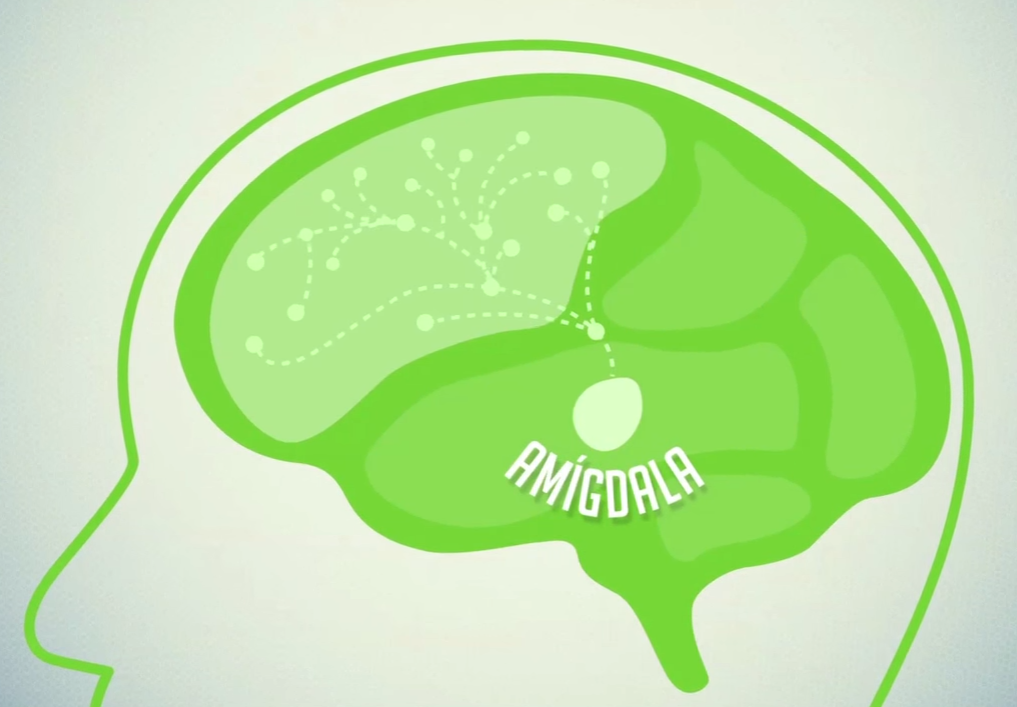
\includegraphics[scale=0.2]{img/cerebrogus.png}
\captionof{figure}{Esquema de la posición de la amígdala en el cerebro humano.}
\end{minipage}

Por simplificar mucho hasta el momento, la parte racional está en el prefrontal y la parte emocional está en la amígdala.


Con esto se explicaría que si estás emocionado con algo, tengas una mejor concentración y por tanto un mejor aprendizaje. En realidad, el cerebro tiene muchas partes y para que el proceso de aprendizaje sea total se deberían emplear todas las regiones y funciones del cerebro.


Como dijo \textbf{Helena Lopez Casares en la conferencia que dio el 20 de septiembre en el Campus Vicálvaro} sobre inteligencias múltiples, hay estudios que demuestran que personas con problemas en la parte del cerebro que controla las emociones son incapaces de tomar una decisión, con lo cual se demuestra la importancia de todas las partes del cerebro deben estar activas y conectadas.

\paragraph{Educación bulímica. Matemáticas, Historia y Filosofía}
Me ha gustado mucho la afirmación que hace Javier Blumenfeld: “Tenemos una especie de educación bulímica: yo te meto contenidos y tú me los vomitas en el examen”. Esto es lo que yo llamo metodología tradicional de la enseñanza.


En este caso sí haría diferenciación por asignaturas y lo aplicaría a mi experiencia personal. En el caso de las matemáticas, aparte de que siempre me han gustado más, he sido capaz de aprenderlas y es muy difícil que se me olviden. O si hay algo que no tengo claro, con un simple repaso sería capaz de recordarlo. Estas matemáticas las he aprendido bajo un contexto de educación bulímica y aun así he sido capaz de aprenderlas. Sin embargo, en asignaturas como historia, filosofía, u otras asignaturas que la manera de aprobar consistía en la memorizar y repetir lo memorizado en el examen, no he recordado nunca nada de adulto.


Sin embargo, es curioso como a día de hoy sí me siento atraído por la historia y por los pensamientos filosóficos. Bajo mi punto de vista es que este cambio se debe a que he alcanzado unos conocimientos y una madurez que me permiten disfrutar de ello. No tenía ningún sentido estudiarlo con la edad que tenía. No disfrutaba de ello. Hace poco hice un tour que te lleva por el Madrid de los Austrias con guía y lo disfruté muchísimo, cosa que era impensable cuando era un niño. Este sería un claro ejemplo de que cuando algo te gusta lo aprendes mejor. Aunque en este caso concreto, tengo la opinión de que es muy difícil motivar a unos alumnos que no han vivido los suficientes años como para entender y disfrutar de la historia y de los filósofos.


\paragraph{Buscando culpables}
En el punto anterior he hecho una exposición desde mi propia experiencia personal. Sin embargo, tengo compañeros y amigos que sí que han sido capaces de aprender más cosas de historia que yo en etapas tempranas de la vida.


¿Cuál será el motivo por el que yo NO he aprendido historia y otras personas que conozco sí? 
¿Será que el colegio en el que ellos estudiaban, fueron capaces de emocionarles mejor en Historia? 
¿O será que yo nunca he puesto interés? 
Tenemos que tener cuidado también con aquellos alumnos que se aprovechen de esto para decir que no han aprendido lo suficiente alegando que el sistema educativo no era el adecuado o que las metodologías de aprendizaje no eran las adecuadas. Hay que hacer analizar todas las situaciones de manera individual para poder discernir aquellos alumnos que realmente han sido sometidos a altos niveles de estrés que han limitado su capacidad de aprendizaje de aquellos alumnos que simplemente no ponían interés.


\paragraph{Entendido el problema. Y ahora …?}
Una vez hecho el diagnóstico de la situación y entendido que como docentes tenemos que motivar para conseguir emocionar al alumnado y de esta manera conseguir que el aprendizaje sea más efectivo, lo que hay que ver ahora es cómo llevar a cabo ese cambio.


Pero antes de empezar a analizar las diferentes alternativas que se plantean como los trabajos por proyectos, aprendizaje basado en problemas, etc me gustaría lanzar una pregunta abierta sin ánimo de criticar estas iniciativas de cambio y es la siguiente, ¿Qué pasaría si con el cambio ocurre que hay alumnos que no se sienten motivados por estas nuevas metodologías? Podríamos volver al problema del cual partimos y volveríamos a tener alumnos desmotivados. Según esto, lo ideal sería una enseñanza personalizada en el individuo y no en el grupo. Pero por otro lado, vivimos en sociedad, somos seres sociales y una enseñanza individual podría dar lugar a perder otro tipo de conocimientos sociales muy importantes. La conclusión es que podamos combinar una educación en la que cada uno aprenda a su velocidad pero en sociedad.

\paragraph{Mens sana in corpore sano}
Me ha interesado mucho también el estudio que asocia deporte con aprendizaje.


Tener alumnos sentados durante tanto tiempo en el aula es antinatural. Después de hacer un ejercicio, sobre todo aeróbica el cerebro funciona mejor.


La irisina se genera al hacer deporte y baja de los músculos al cerebro y favorece la plasticidad neural, que es la base del aprendizaje.


En este caso, las imágenes que aparecen en las transparencias de clase son muy significativas. Se ha evolucionado en muchos aspectos de la vida y sin embargo parece que las aulas permanecen “incambiadas” desde hace muchos años.
\end{opin}


\begin{opin}{\victorcolor}{Víctor}



\subsubsection{Charla de neurodidáctica}

Aunque no es propiamente de la asignatura, es gracias a la profesora, Raquel Garrido,  que fui a la jornada complementaria sobre \textbf{Neuroeducación}.
%
En este charla, además de tratar conceptos como la \textit{amígdala}, comentada por Gustavo anteriormente, tratamos del \concept{TDAH}. 
%
El ponente hacía una reflexión muy interesante: \textit{Se medica para que el chaval con un trastorno neurológico se adaptara al método. 
%
Tal vez el problema no está en el trastorno neurológico sino en la metodología empleada.} para concluir un poco después: \textit{Con la manera de dar clase se puede contrarrestar totalmente el TDAH de un alumno.}
%
Esta reflexión me hizo también ser consciente de la importancia que tiene mi labor. 
%
De hecho, nos contaba un caso de su clínica en el que un chaval tendría que ser medicado si le tocaba el profesor de Matemáticas A pero se podría evitar la medicación si su profesor de Matemáticas era B, porque así había sido otros años. ¡Qué responsabilidad!

En esta charla se dió una clave muy importante para tratar con alumnos con TDAH:\textit{
Hay una diferencia entre no aprender y aprender pero no ser capaz de retomar ese conocimiento aprendido. 
%
Una persona con TDAH puede aprender, pero su frontal no es capaz de retomar la información.}

Por último, resumo otra idea que me resultó esclarecedora:
%
Atender es un acto involuntario, la concentración es consciente. 
%
No podemos pedir que nos presten atención (porque es involuntario). Necesitamos captar su atención. 
%
Por otro lado,
la concentración es la selección voluntaria de uno de los focos a los que atendemos. 
%
Sí podemos pedirles que se concentren en lo que estamos haciendo, ya que eso sí depende del alumnado.




\end{opin}

\begin{opin}{\pedrocolor}{Pedro}

.


\end{opin}

\begin{opin}{\virgicolor}{Virginia}
.


\end{opin}


\subsection{Introducción a la Neurodidáctica (Tema 2.2 - 24/10/2016)}
\begin{opin}{\guscolor}{Gustavo}
.


\end{opin}

\begin{opin}{\victorcolor}{Víctor}
.


\end{opin}

\begin{opin}{\pedrocolor}{Pedro}

.


\end{opin}

\begin{opin}{\virgicolor}{Virginia}
.


\end{opin}


\subsection{Innovación y recursos educativos (Tema 3.1 - 24/10/2016)}
\begin{opin}{\guscolor}{Gustavo}

\subsubsection{Divulgación de las Matemáticas como docentes}

En la clase de hoy Raquel hizo referencia a un debate que puede generar polémica. El asunto es si las matemáticas son asequibles para todo el mundo o solo para elegidos como algunos piensan. Raquel es partidaria de que todo el mundo podría aprender matemáticas correctamente si estas se explican cómo deberían. En mi opinión, yo no afirmaría ni una cosa ni la otra al 100\%, es decir, no todo es blanco ni negro. Relacionándolo con las inteligencias múltiples que explicó Helena López Casares en la conferencia que dio el 20 de septiembre en el Campus Vicálvaro, me atrevería a decir que un profesor puede intentar despertar el interés de un alumno por las matemáticas, pero es cierto que dentro de todas las posibles inteligencias que pueden existir, si un alumno no tiene bien desarrollada la inteligencia relacionada con las matemáticas, un profesor podrá ser capaz de despertasr el interés de un alumno hasta un límite.

En cualquier caso, ya sea para difundir las matemáticas a todo el mundo o no, lo que está claro es que hay que intentar quitar ese estigma existente dentro del mundo matemático acerca de que la gente a la que le gustan las matemáticas son “bichos raros”. Para ello hay que difundir y divulgar las matemáticas y qué mejor manera que hacerlo de un tiempo a esta parte que a través de la prensa y de los medios de comunicación. 

El problema está en que los periodistas históricamente han huido de las matemáticas desde bien entrada la Universidad y por tanto existen muchos errores en prensa y televisión acerca de las matemáticas como se pueden ver en las transparencias de clase o en el video visto en clase de Marilo Montero (\url{https://www.youtube.com/watch?v=zclITKd4ivQ}). Este error tiene que ver con el error o fallo que puede existir a la hora de representar ciertas expresiones matemáticas como puede ser la expresión 48/2(9+3) y que ha generado un debate en los foros de la asignatura que muestro a continuación dado que  me pareció muy interesante y no tuvimos tiempo para abordarlo en clase

En mi opinión, inicialmente el resultado era 2, clarísimamente. Pero después de razonar con mis compañeros de clase vi que podría haber más soluciones aparte de la mia. David Soria explicó lo siguiente: 

\begin{mdframed}
El problema tiene dos opciones distintas dependiendo del orden de operación. Hay dos elementos de distinto orden que son PEMDAS Y BEDMAS, según en la escuela que te hayan enseñado puede ser uno u otro. El orden para aplicar las operaciones en PEMDAS (Paréntesis, Eponenciación, Multiplicación, División, Adición y Sustracción) mientras que el orden en BEDMAS (Paréntesis,, Exponenciación, División, Multiplicación, Adición y Sustracción). 

Con PEMDAS el resultado de la operación sería item 

\[
48÷2·(9+3) \to 48 ÷ 2·(12) \to 48÷2·12 \to 48÷24 = 2
\]

Con BEMDAS  el resultado de la operación seria item 

\[
48÷2·(9+3) \to 48 ÷ 2·(12) \to 24·12 = 288
\]

\end{mdframed}

Antonio Jesus Guerrero y Carlos Rodiño entendían que “que multiplicar y dividir están al mismo nivel, igual que sumar y restar; y que en tal caso la prioridad de operación es de izquierda a derecha.”

Posteriormente, Manuel Pulido compartió su forma de pensar con Carlos y con Antonio,  y además corroboró la información con un libro de texto indicando que es la manera más extendida de hacerlo.

El libro de texto decía lo siguiente:

\textit{En general:}

\begin{itemize}
\item \textit{En operaciones con paréntesis, primero hay que realizar las que están entre paréntesis y luego las demás.}
\item \textit{En operaciones sin paréntesis, primero se efectúan las multiplicaciones y divisiones y luego, las sumas y las restas.}
\item \textit{En operaciones de igual prioridad, primero la de más a la izquierda.}
\end{itemize}

\textit{Por lo tanto ellos lo calcularían así:}

\[
48÷2·(9+3) \to 48 ÷ 2·(12) \to 24·12 = 288
\]



Por último, intenté llegar a una conclusión que es la importancia que tiene como colocar las expresiones matemáticas para no dar lugar a ambigüedades de este estilo.


Lo que queda claro es que unos entienden la expresión como $\frac{48}{2(9+3)}$ y otros como $\frac{48}{2}(9+3)$.

Si ambas expresiones se reflejaran así no daría lugar a ninguna confusión.

En cualquier caso no estoy de acuerdo en aplicar las reglas que indican ciertos libros de texto dado que si aplicamos estas reglas indicadas por el libro de texto al que hacía referencia Manual, la expresión 

Podría interpretarse como si fuera igual a 288, cuando todos tenemos claro que debe ser igual a item 

Para terminar el debate Miriam Expóstio indicó que 
\textit{Desde mi punto de vista, para que se entendiese que hay que dividir todo entre "2(9+3)" se tendría que poner todo ese término entre corchetes, no?}


Con lo que estoy totalmente de acuerdo. Y por tanto, al no haber corchetes, el problema lo tiene quien escribe la expresión al haber varias interpretaciones.
Las matemáticas deben ser exactas y no dar lugar a interpretaciones. Para interpretaciones ya están las leyes ;-)
Además de los errores cometidos por los periodistas de manera involuntaria como puede ser el de Mariló también están los errores cometidos intencionadamente con el objetivo de manipular a esa parte de la sociedad menos documentada. Ejemplos pueden ser el número de asistentes a una manifestación que varía en función de diversos intereses.
También hablamos acerca de los errores comunes que tienen los alumnos a la hora de realizar ciertas operaciones básicas en matemáticas y que independientemente de ser de letras o de ciencia, no se deberían cometer. Es como si los de ciencia dijeran que no saben escribir gramaticalmente bien porque son de ciencia. No tiene sentido. La cultura es independiente de ser de ciencias o de letras.
Otra de las formas de divulgar las matemáticas en televisión es a través de series. Por ejemplo:

\begin{itemize}
\item “Universo matemático” era una serie, producida en el año 2000, que constaba de 10 capítulos y que abordaba distintos temas relacionados con la matemática. La obra obtuvo en el año 2002 el Premio a la divulgación científica del Festival Internacional Científico de Pekín. 
\item Se puede ver en 
\href{http://www.rtve.es/alacarta/videos/universo-matematico/} {http://www.rtve.es/alacarta/videos/universo-matematico/} 
\item “Más por menos”. Esta serie consta de 13 programas emitidos de septiembre de 1996 a enero de 1997 y de noviembre de 2002 a enero de 2003 en el programa de Televisión Educativa de TVE-2 "La Aventura del Saber".
\item Se puede ver en 
\href{http://www.rtve.es/television/la-aventura-del-saber/documentales/mas-por-menos/} {http://www.rtve.es/television/la-aventura-del-saber/documentales/mas-por-menos/} 
\item “Orbita Laika” sección de Matemáticas por Raúl Ibañez.
\item Matemáticas invisibles:
\begin{itemize}
\item Curiosidad sobre el tamaño de las hojas DINA-n (
\href{http://www.sabercurioso.es/2008/11/05/por-que-una-hoja-de-papel-din-a4-tiene-el-tamano-que-tiene/}{http://www.sabercurioso.es/2008/11/05/por-que-una-hoja-de-papel-din-a4-tiene-el-tamano-que-tiene/}
)
\item Explicación del digito de control de un código de barras. Todo tiene su explicación
\end{itemize}
\end{itemize}



Como vemos, hay muchas formas de divulgar las matemáticas y nosotros como futuros docentes debemos ser parte fundamental en el futuro de esta divulgación, ya sean:

\begin{itemize}
\item Artículos en revistas  
\item Convocatorias de actividades relacionadas con las matemáticas (fotografía, concursos, juegos…)
\item Concesiones de premios (Medalla Fields) 
\item Iniciativas como dar publicidad a los congresos internacionales de matemáticas 
\item Promover jornadas de popularización y divulgación  (“olimpiadas matemáticas”) 
\item Museos (Museo Nacional de Ciencia y tecnología, MUNCYT, antiguo Cosmocaixa)) 
\item Páginas web divulgativas
\item Divulgamat (
\href{http://www.divulgamat.net/}{http://www.divulgamat.net/}
)
\end{itemize}

\begin{minipage}[hbtp]{1.0\linewidth}
	\centering
	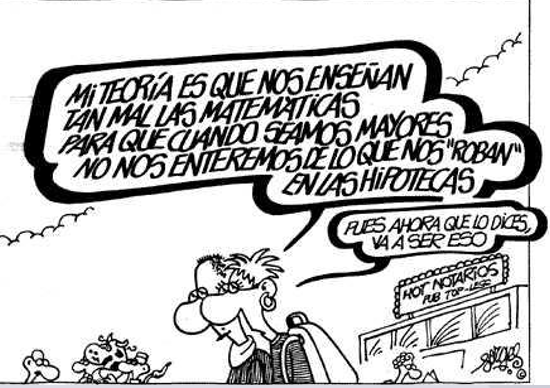
\includegraphics[width=0.6\linewidth]{img/chistegus.png}
	%\captionof{figure}{Coche de mediadios del siglo pasado.}
\end{minipage}

\end{opin}






\begin{opin}{\victorcolor}{Víctor}

En mi diario incluía también una mención sobre el ejemplo $48÷2·(9+3)$ tratado por mi compañero Gustavo, pero lo voy a omitir por evitar repeticiones innecesarias.

\subsubsection{Docentes como divulgadores}

Me ha resultado muy novedosa la idea de que \textit{los profesores deberíamos ser los primeros divulgadores de las Matemáticas} (Antonio Durán). 
%
No sólo en el aula con los alumnos, sino también fuera de ella.
%
Hacen falta personas apasionadas por las Matemáticas, capaces de ayudar a la gente a romper el mito ``Es que soy de letras'' 
%
\footnote{Al igual que personas apasionadas por las letras que rompan con el mito ``Es que soy de ciencias''. Qué pasa, ¿que por ser de ciencias no saber redactar ni expresarte por escrito?}
%
Y a veces, ese argumento se utiliza para escaquearse de llevar las cuentas en un viaje o en una cena, cuyos cálculos no pasan de simples divisiones y sumas que un estudiante de 5º de Primaria podría hacer.

\subsubsection{Construyendo el conocimiento matemático sin lagunas}

En verano estuve de voluntariado en Perú y una semana fue dar clase de mates a chavales de secundaria de allí. 
%
Les ocurría que sabían despejar las ecuaciones perfectamente. Hacían todos los pasos bien, hasta que al llegar al final, $3x = 24 \to x=\frac{24}{3} = ?$. 
%
El último paso no eran capaces de hacerlo. ¿Cómo es posible que lleguen al curso en el que están y sepan despejar sin saberse las tablas de multiplicar? 
%
¡Qué sistema educativo tan ineficiente! 
%
Pasan de curso sin los conocimientos necesarios... construyen el conocimiento con unas lagunas bestiales.

Viendo los errores de primero de grado propuestos por Raquel me doy cuenta que no hay tanta diferencia entre el modelo de allí, con el modelo de aquí; 
%
en cuanto a construir un conocimiento sólido sin lagunas.


La Ted Talk de Salman Khan me parece una charla que todo docente de Matemáticas debería ver (tanto es así, que mi primera aportación a los foros de la asignatura fue plantear esta charla).
%
¿Te imaginas construir el tejado de un edificio sin haber terminado los cimientos?
%
Nadie trabaja así. Ni siquiera nadie, exceptuando a Fito y Fitipaldis, sugiere trabajar así.
%
¿Porqué en Matemáticas enseñamos a integrar sin que se haya interiorizado bien la derivada? ¿Porqué tratamos de enseñar diagonalizar matrices sin que los alumnos tengan claro cómo se factoriza un polinomio con Ruffini?
%
No digo que haya que enseñar Ruffini en la universidad, sino que los docentes en la secundaria nos esforcemos por no dejar lagunas en el conocimiento de los alumnos. 
%
``Enseñar para la maestría'', como dice Salman Khan.

\paragraph{Khan Academy}

Al hilo de retomar esta charla este curso (ya la conocía anteriormente) estuve paseando por la web y viendo los recursos que tienen.
%
Es una pena que esté en inglés y tal vez no sea utilizable en clase, pero ayuda a hacerse una idea de cómo funcionar. 
%
Además, están trabajando en traducciones, para hacer llegar la academia a más países.

Otro aprendizaje, al hilo de Khan, es la importancia del inglés. 
%
Más allá de poder comunicarse, en internet hay infinidad de recursos (empezando por las charlas Ted) que merecen mucho la pena y que se podrían estar aprovechando mucho más, si supiéramos inglés.
%
A raíz de esto, cuando me preguntan qué es lo que más valoro del inglés, lo que siempre contesto es: ``poder aprender autodidactamente de lo que sea en internet y acceder a reflexiones y conocimiento de otras personas''.


\end{opin}

\begin{opin}{\pedrocolor}{Pedro}

\subsubsection{La clase invertida - jornada complementaria}
\vspace{2.0cm}
\end{leftbar}
\vspace{-2.0cm}
\begin{figure}[hbtp]
\begin{leftbar}{\pedrocolor}
\vspace{1cm}
\centering
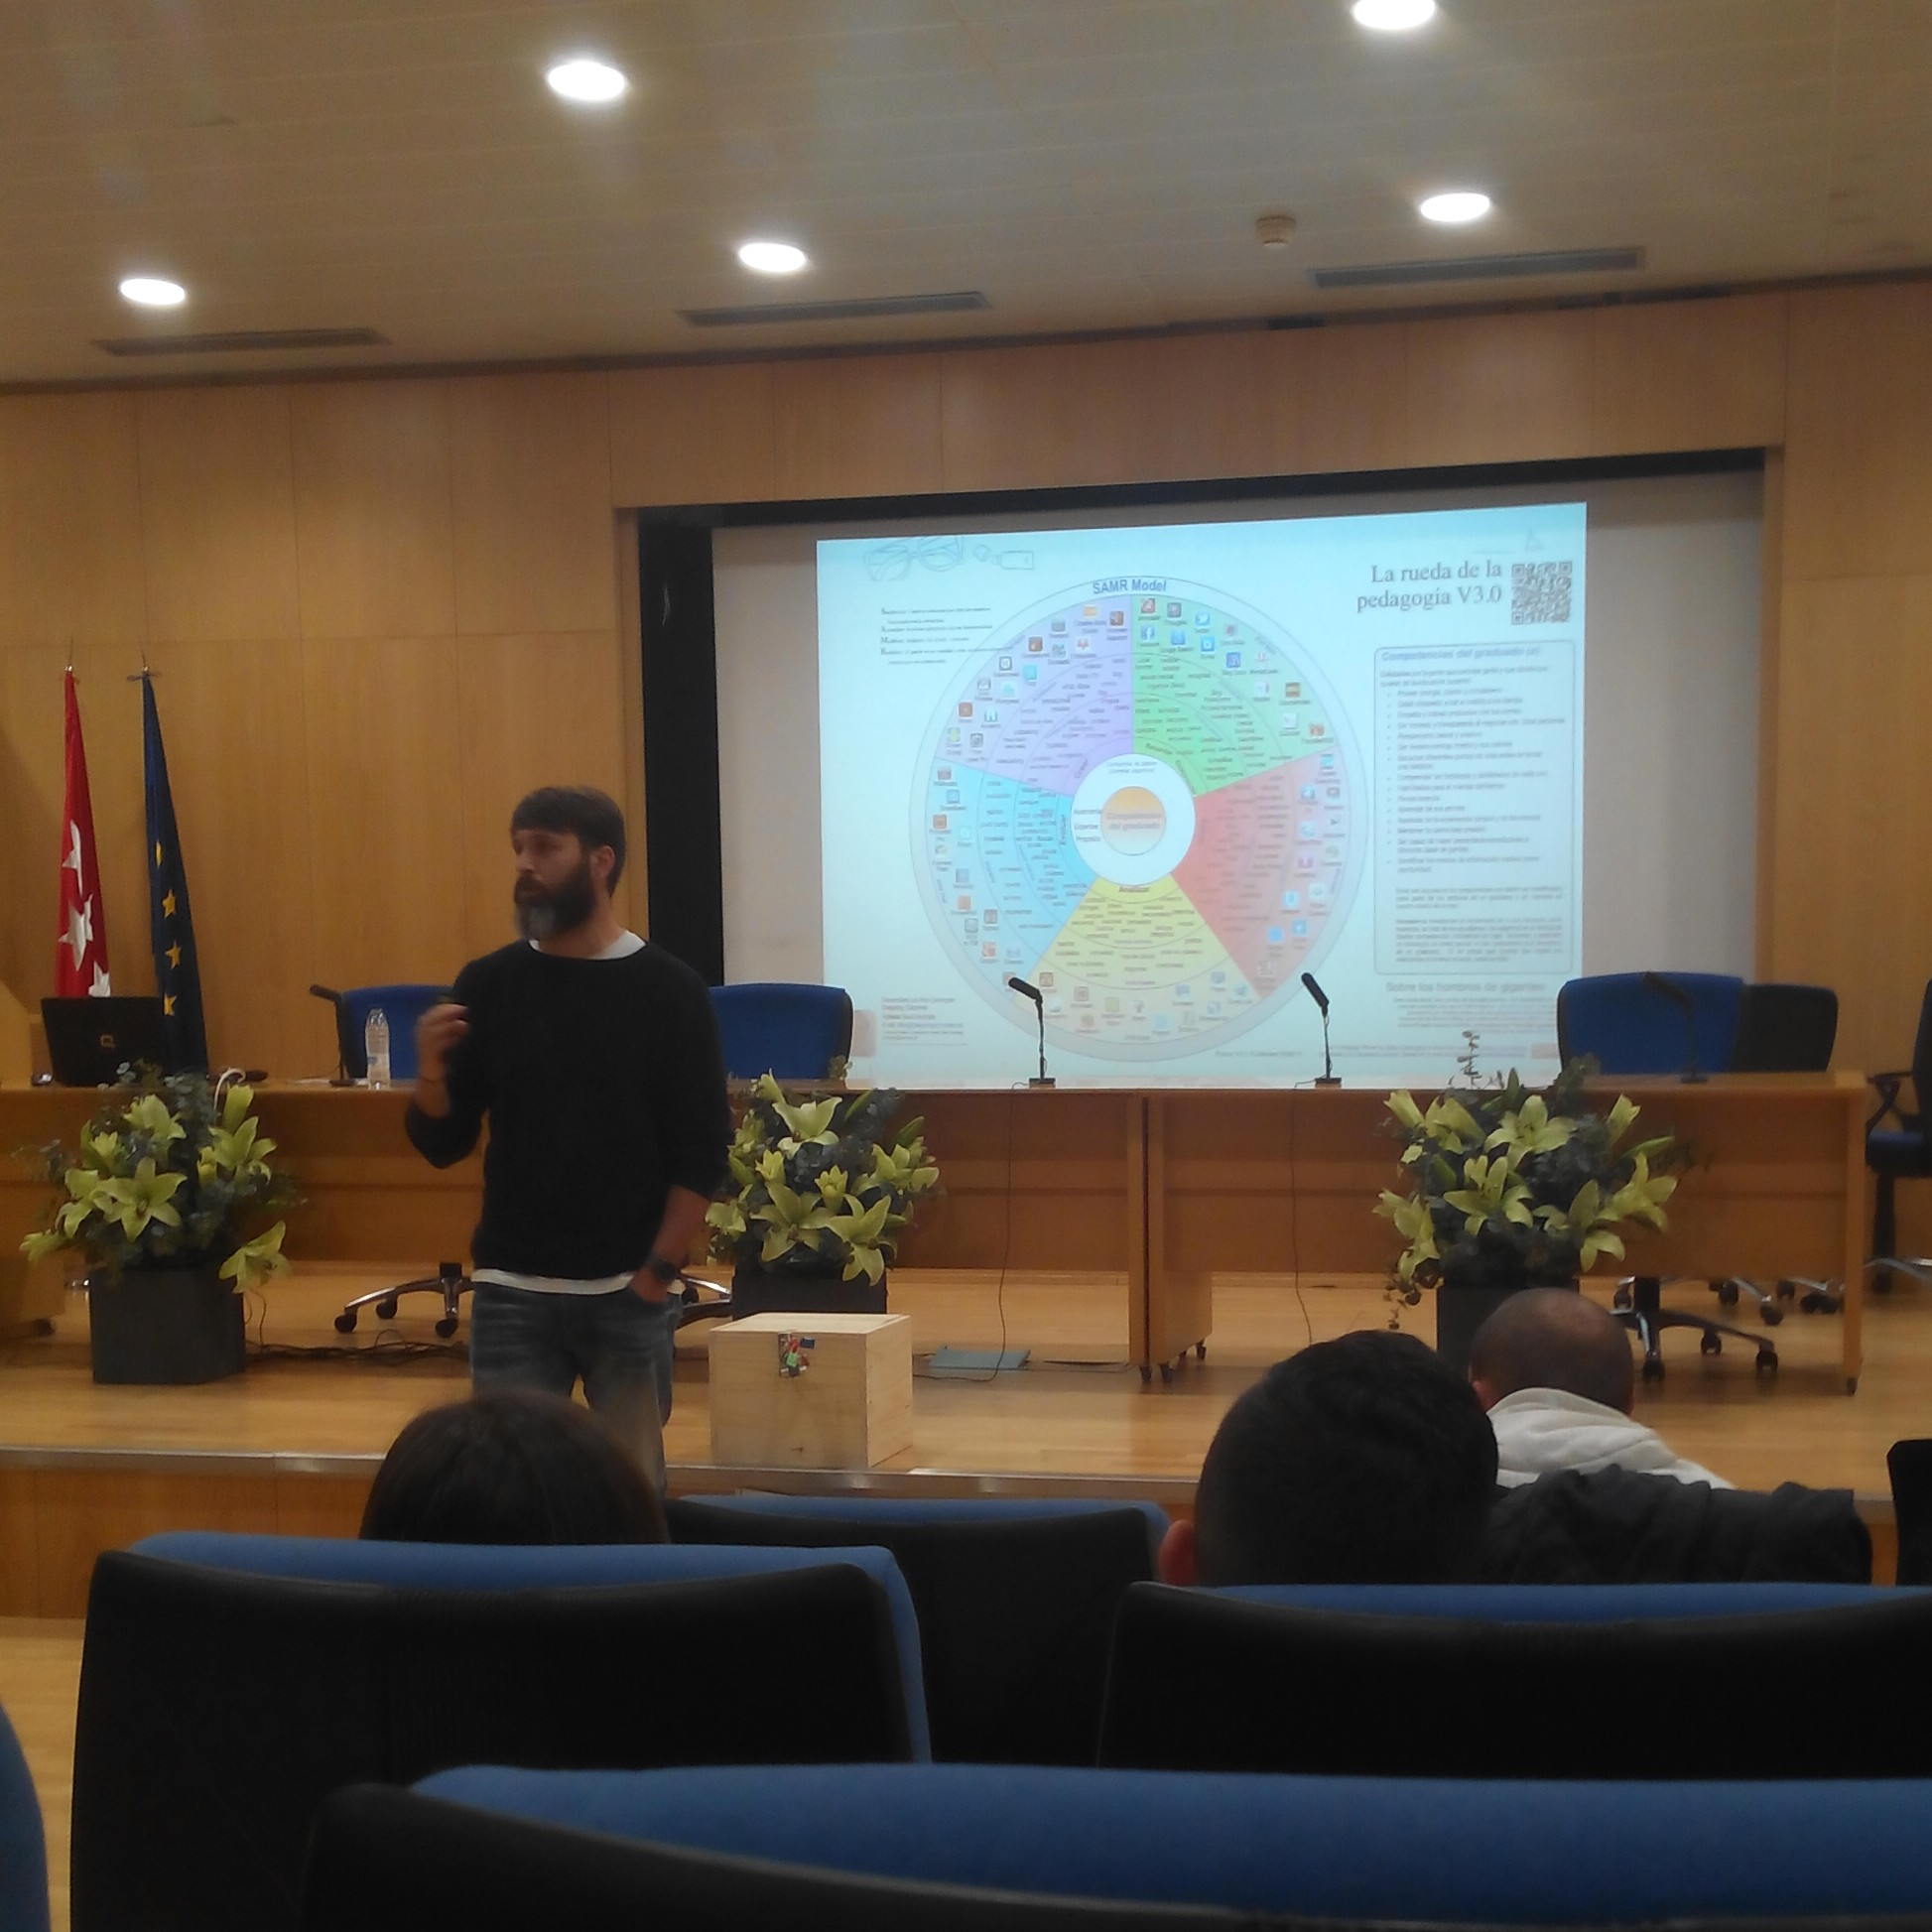
\includegraphics[scale=0.12]{img/pedron.jpg}
\caption{Comienzo de la ponencia.}
\vspace{2.0cm}
\end{leftbar}
\vspace{-2.0cm}
\end{figure}
\begin{leftbar}{\pedrocolor}

\textbf{Jonathan Bergmann y Aaron Sams}, dos profesores de química, acuñaron el término de “Flipped Classroom”. En un principio estaba orientado para aquellos alumnos que frecuentemente faltaban a clase por algún motivo personal. Con el tiempo se dieron cuenta que este mismo modelo permitía que el profesor centrara la atención en las necesidades individuales de aprendizaje de cada estudiante.

Para poder entender en qué consiste esta metodología activa de “Flipped Classroom”, Chema nos hizo llegar la siguiente definición de Raúl Santiago:

Modelo pedagógico que transfiere el trabajo de determinados procesos de aprendizaje  fuera del aula y utiliza el tiempo de clase, junto con la experiencia del docente, para facilitar y potenciar otros procesos de adquisición y práctica de conocimientos dentro del aula. 

En pocas palabras: “Lleva tu clase a cada estudiante, en cualquier momento y en cualquier lugar”

Pero la pregunta que surgió era, ¿Cómo se controla si tus alumnos hacen su trabajo fuera del aula? Chema habló que era fundamental explicar a los alumnos en qué consistía eso de la clase invertida y lo importante que es seguir unos patrones  para alcanzar el éxito que se traduce en “aprendizaje”. Según sus palabras, ellos tienen que saber que son los protagonistas de su propia película. Todos pensamos que estas palabras sobre el papel suenan bien, pero la verdad resultante en el aula es bien distinta, la prioridad de los alumnos no es aprender. Ante esto, nos presento algunas herramientas como \textbf{Playposit y EDpuzzle}:

\begin{itemize}

\item  \textbf{Playposit} El profesor puede incluir preguntas dentro de un vídeo (de origen propio o de YouTube). Lo novedoso es que el estudiante tiene que contestar primero las preguntas antes de poder continuar y sin poder avanzar a partes que todavía no ha visionado (si puede rebobinar y luego avanzar). Por otra parte el profesor puede ver en su tablero que estudiantes han realizado la tarea y los resultados. Material muy útil para utilizar en clase invertida. 

\item  \textbf{EDpuzzle} Permite convertir cualquier video en tu propia lección educativa de una forma rápida y fácil. De este modo podremos cortar un video si nos interesa solo una parte, grabar nuestra propia voz encima del video.  El resultado serán videos muy interesantes y entretenidos. 
\end{itemize}

Personalmente creo que son dos herramientas muy bien pensadas para educadores. Playposit me permite poder evaluar a mis alumnos de manera individual, identificando sus puntos débiles sobre un determinado temario.

 
A continuación, Chema nos habló de los 10  errores más comunes a la hora de crear una Flipped Classroom:

\begin{itemize}

\item Videos demasiado largos ( Un minuto por año que tenga el alumno aproximadamente) 

\item Añadir más que remplazar. Los videos deben remplazar el contenido del texto, no añadir más. 

\item Dar clase cuando los alumnos no atienden. Al principio será necesario ver los vídeos en el aula, ya que normalmente les costará cambiar de rutina. 

\item Elaborar contenido de difícil acceso. Utilizar solo un soporte para elegir los videos y materiales. Explicar donde está todo alojado y cuál es su funcionamiento. Hacerlo fácil. 

\item Inactividad de los profesores en el aula. El profesor no deberá estar cómodamente sentado durante la clase. Deberá resolver dudas de los alumnos. 

\item Rendirse. Si el método no funciona, cambia de método. 

\item No tener en cuenta los alumnos con dificultades. 

\item No hacer clases interactivas. 

\item Utilizar videos de otras personas. Hay que personalizar los videos para tus alumnos. 

\item No hacer las clases divertidas y amenas. 
\end{itemize}
Me he querido centrar en esta metodología porque opino que permite al alumno marcar su ritmo de aprendizaje. Nos alejamos de los patrones que marca el sistema educativo actual, que hace que unos alumnos vayan con la lengua fuera, mientras que otros se aburren en clase. Aquí cada alumno elige su momento de estudio.




\end{opin}

\begin{opin}{\virgicolor}{Virginia}

\subsubsection{Divulgación de las matemáticas como docentes}

En este tema vimos la importancia de la correcta divulgación de las matemáticas.  Recalco lo de correcta porque de nada sirve divulgar matemáticas si está no se hace bien y por desgracia en los medios de comunicación se cometen errores bastante importantes. Teniendo en cuenta que los principales medios de divulgación son tales medios de comunicación como, televisión, periódicos, radio e Internet creo que es de vital importancia evitarlos: ¿cómo podemos pretender que los niños se expresen bien o les exijamos unos conocimientos básicos en matemáticas si los propios periodistas cometen fallos tremendos? Uno de los ejemplos que puso Raquel y que me dejo boquiabierta fue el de Marilo con el índice de masa corporal, ya no por el hecho de que no sea capaz de usar una calculadora aun cuando le estaban explicando paso a paso como hacerlo, sino de la propia imagen que da de desinterés y despreocupación como si no pasara nada el ser incapaz de hacer algo tan sencillo como una potencia y una división.

En mi opinión, el problema con las matemáticas empieza desde pequeños en el colegio donde comienzan a percibir la asignatura como algo difícil y aburrido. Para ello la labor del profesor es de vital importancia desde las primeras etapas del aprendizaje, de forma que tiene que ser capaz de establecer una conexión entre las emociones de los alumnos y la utilidad de las matemáticas en la vida real. A día de hoy con los avances de la tecnología creo que es más sencillo ya que existen multitud de juegos matemáticos o mentales que se usan en tablets y spmartphones y que los niños estarían encantados de utilizar.

A parte de la labor del profesor, como he comentado antes, los medios de comunicación son la principal fuente de información por lo que la divulgación por parte de los mismos es imprescindible para que llegue a las distintas edades. Es cierto que existen cada vez más programas relacionados con la ciencia y las matemáticas como el Hormiguero, Orbita Laika y Desafía tu Mente. Si bien el hormiguero es un programa de éxito porque lleva famosos de distintos campos y tiene diferentes secciones el programa, los otros dos programas me temo que su audiencia dista mucho de lo que tendría que ser y más sin los comparamos con programas basura como Gran Hermano o Mujeres Hombres y viceversa.  Es una pena que la gente se una más para ver programas basura que un programa de divulgación. Siempre escucho que si lo ponen es porque la gente ve esos programas, pero también pienso que, si desaparecieran todos esos programas basura y se pusieran más programas de entretenimiento relacionados con la ciencia y su divulgación y en un horario más apto para niños, seguro que se crearían unas inquietudes diferentes a esos niños, tendrían más ganas de aprender cosas curiosas e interesantes que buscar la forma de ganar más dinero trabajando menos.

Dentro de los libros, videos y/o artículos de divulgación matemática que vimos en clase quiero destacar los siguientes:

\begin{itemize}

\item La sección de Raúl Ibánez sobre matemáticas en Orbita Laika ya que Raúl consigue ganar el premio más importante de divulgación científica en España. Además es el creador y director de una página muy interesante, Divulgamat: \url{http://www.divulgamat.net/} 

\item Universo matemático que fue galardonada en el Festival Internacional Científico de Pekín con el Premio a la divulgación científica. 

\item El libro de Mateschef ya que el libro trata de hacer relaciones curiosas entre geometría y cocina, y las matemáticas y la cocina son dos cosas que me encantan así, que mejor forma que unir las dos. En el campo de la cocina y teniendo en cuenta el nombre de este libro, recuerdo siempre como en el programa de MasterChef cuando hacen postres recalcan siempre que “la repostería es matemática pura”. 

\item Matemáticas invisibles: muy interesante el artículo de las plantas carnívoras: \url{http://www.agenciasinc.es/Noticias/Las-plantas-carnivoras-utilizan-las-matematicas-para-cazar-a-sus-presas} 

\item El mundo con mirada matemática: a parte de lo que vimos en clase me gustaría añadir una web en la que se incluyen edificios famosos inspirados en las matemáticas: \url{http://www.metrocuadrado.com/noticias/especiales/edificios-famosos-inspirados-en-las-matematicas-664} 
\end{itemize}


Además de todos los libros que vimos en clase de los distintos divulgadores y todos los programas de los que hablamos, me gustaría aportar otros programas que yo he visto y que me parece muy interesantes como son: Mythbusters (Cazadores de mitos), por el Discovery Channel, y Brain Games (Juegos mentales) por National Geographic. El primero, está más relacionado con la divulgación científica y consistía en comprobar la veracidad de las leyendas urbanas y otras creencias usando para ello métodos científicos. El segundo, en realidad podría haberlo incluido cuando se trató la neurodidáctica ya que en este programa se explora los componentes del cerebro humano y su funcionamiento empleando expertos en ciencia cognitiva, neurociencia y psicología. No obstante, son dos programas muy interesantes a la vez que entretenidos, por lo que habría que promocionar más este tipo de programas.

A parte de todos los divulgadores que comentó Raquel quiero hablar de Eduardo Sáenz de Cabezón, un matemático que intenta relacionar las matemáticas con la magia y el humor. Además, es uno de los participantes de un grupo de matemáticos, biológos, científicos... que hacen monólogos. Aquí muestro el link de dos noticias sobre él y las matemáticas:

\url{http://www.abc.es/sociedad/abci-eduardo-sanchez-cabezon-matematico-desvela-magia-numeros-201512180154_noticia.html}

En este artículo Eduardo reflexiona acerca de la tendencia de la gente a renegar de las matemáticas: “Quizá solo falta perderles el miedo, acercarse de forma diferente a la que estamos acostumbrados”.

\url{http://www.nacion.com/vivir/ciencia/hombre-saca-chistes-matematica_0_1565443465.html}

En el vídeo que sale en este artículo me parece divertido su consejo para hacer un regalo a alguien que le quieres demostrar que tu amor es para siempre: “Si quieres decir a alguien que le quieres para siempre, regálale un teorema en lugar de un diamante”. Para finalizar recalca que hay que cambiar la educación matemática actual.

Y por último la página del grupo de monologuistas al que pertenece y de las actividades que realizan que me parece una labor muy importante, interesante y divertida para dar a conocer los diferentes entresijos de la ciencia:

\url{http://www.bigvanscience.com/tbvt.html}

En definitiva, hay multitud de formas de disfrutar de la ciencia en general y las matemáticas en particular, y para hacer uso de dichas formas, el deber de padres, profesores y medios de comunicación es conseguir inquietar y emocionar las mentes de los niños, para lo que antes son los propios adultos los que tendrían que conseguir emocionarse.

\end{opin}


\subsection{Clase cancelada (31/10/2016)}

\subsection{Pizarras digitales (Tema 4 - 07/11/2016)}
\begin{opin}{\guscolor}{Gustavo}


El objetivo que pretende Manuel es el de concienciarnos de la utilidad práctica que tiene el uso de las pizarras digitales en el aula a la hora de la enseñanza.

Manuel indica que las claves para que algo tenga éxito en educación son 3:

\begin{itemize}
\item[1.]Que sea muy fácil. 
\item[2.]Que sea adaptable. Valido para cualquier asignatura. 
\item[3.]Que sea útil pedagógicamente. 
\end{itemize}

\subsubsection{Hoy Soy Feliz Porque Tengo Ayuda}

\textbf{H}oy \textbf{S}oy \textbf{F}eliz porque tengo \textbf{A}yuda.

El camino para conseguir ese éxito tiene que ver con el título del apartado.

\paragraph{H de Hardware}
Son las herramientas. Pero el importante es el que transmite que es EL PROFESOR. Tipos de hardware:

\begin{itemize}
\item Pizarra Digital Interactiva (PDI) 

\item Pizarra Digital Interactiva Portátil (PDiP). La que usa el profesor en su clase. Se puede usar desde cualquier lugar. Más económica, más flexible y con mayores posibilidades. 

\item Articlick. EVCD: Evaluacion continua Digital. 

\item Cámaras de documentos. Es barata y permite ver documentos y hacer anotaciones sobre ellos. 

\item Micrófonos y altavoces. 
\end{itemize}

\paragraph{S de Software}
Hay muchos tipos de software.

Las características del software asociado a la pizarra que nos mostró el profesor incluía:

\begin{itemize}
\item Una barra de herramientas personalizable y flotante sobre cualquier aplicación.  

\item Se permiten hacer anotaciones. Todas las anotaciones se guardan automáticamente.  

\item Se puede borrar lo que se quiera.  

\item Se pueden exportar a cualquier formato.  

\item Se puede guardar un video con sonido de cualquier explicación previo a darle a guardar. 

\item El lápiz hace de ratón: 
\begin{itemize}

\item Boton izquierdo: Punta 

\item Doble click: Botón central 

\item Botón derecho: último botón. 
\end{itemize}
\end{itemize}

Una vez explicadas las capacidades de la pizarra, Manuel nos mostró una serie de ejemplos de aplicación de simulaciones de mucha utilidad entre las que destacaría la “Graphing  calculator 3D” por encima de todas las demás ya que siempre cuesta mucho explicar cómo se representan los planos en el espacio y esta herramienta es absolutamente fantástica. Otras aplicaciones que también me resultaron interesantes fueron:
\begin{itemize}
\item[1.]La aplicación que te permite hacer simulaciones de caída de objetos y un péndulo. 

\item[2.]RM Easiteach con la que explica el movimiento de la tierra con respecto al sol y de la luna con respecto a la tierra. 

\item[3.]Otra aplicación explica los colores primarios y su mezcla que produce los colores complementarios que son los de la impresora 
\end{itemize}

\paragraph{F de Formación}
El profesor tiene que tener un curso presencial motivador

Tiene que existir un curso online

\paragraph{A de Ayuda}
Tienen que existir tanto el apoyo como las ayudas al profesor. IMC

\index{EVCD}\textbf{EVCD}: Evaluacion continua Digital
Por último, hicimos una demostración en clase pasa a explicar la evaluación continua con el programa VPAD. Encontré esta aplicación superútil dado que se pueden hacer evaluaciones interactivas de mucha utilidad.

Además añadiría que no hace falta descargarsela desde el móvil ya que se puede utilizar desde cualquier cliente web.

Hay otros programas como Flow, Plickers y Kahoot en internet en los que también se pueden hacer evaluaciones interactivas.

\paragraph{Street View y realidad virtual de una casa}
Con Manuel también aprendí que con el Street View de Google se puede hacer una foto de una habitación de casa y luego verla con unas gafas de realidad virtual o directamente con un móvil con visión de 360º. Sencillamente impresionante


\end{opin}

\begin{opin}{\victorcolor}{Víctor}

Hoy hemos visto utilizar una \index{PDi(P)}\textbf{PDi(P)}\textbf{ - Pizarra Digital interactiva (Portátil)} y unas cuantas aplicaciones muy útiles para trabajar con tics en el aula.

Entre ellas: Graphing calculator 3D (para dibujar superficies e intersecciones de superficies).
%
Esta herramienta complementa muy bien a geogebra, puesto que los problemas de geometría de segundo de bachillerato son en tres dimensiones y geogebra no tiene opción a dibujar en 3 dimensiones.

Otra herramienta simulaba el comportamiento de objetos atraídos por la fuerza de la gravedad. 
%
Lo primero es dibujar los objetos sin gravedad. Después, al activar la gravedad los objetos se mueven y se puede ver el comportamiento de un péndulo, de un lanzamiento vertical y estudiar a qué altura llega... ¡Los enunciados de los problemas pueden ser vídeos!

A la hora de dibujar en matemáticas, estas herramientas son geniales. Ayudan a visualizar mucho mejor y sobretodo, ahorran mucho tiempo de hacer los dibujos.

La explicación sobre los colores primarios de 15 segundos es la mejor explicación que he escuchado en la vida. 
%
Tener el \textit{flash} sobre los colores primarios de la luz permite mezclaros en el momento y moverlos sin apenas esfuerzo. 
%
Al mezclarlos, se comprueba claramente que son los colores complementarios (los colores que utilizan las impresoras para conseguir todos los demás).

Ha sido muy constructiva esta sesión, aunque hubiera estado mejor poder probarlas, ya que escribir sin mirar a dónde estás escribiendo no me parece algo muy intuitivo. 
%
¿Cuánto entrenamiento hace falta para acostumbrarse?
%
¿Cómo es la curva de aprendizaje?


\end{opin}

\begin{opin}{\pedrocolor}{Pedro}


Esta sesión ha resultado realmente enriquecedora. Ha sido mi primera aproximación a las pizarras digitales gracias a Manuel García. Su gran capacidad de síntesis me permitió tener una visión general de los cuatro campos que cubren las pizarras digitales: Hardware, Software, Formación y Ayuda.

\begin{itemize}

\item \textbf{Hardware:}
\begin{itemize}

\item \textbf{PDIP} (Pizarra Digital Interactiva Portátil). Nos ha mostrado la facilidad de utilización en el aula. Permite poder impartir clase desde cualquier sitio de la sala, cedérsela a los alumnos, y con posibilidad de conectar entre si hasta 9,  simultáneamente repartidas por la clase. 

\begin{minipage}[hbtp]{1.0\linewidth}
\centering
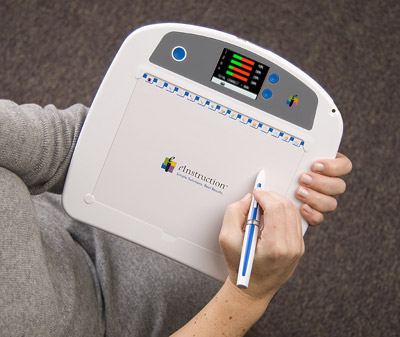
\includegraphics[scale=0.4]{img/pdipedro.jpg}
\captionof{figure}{Pizarra Digital Interactiva Portátil}
\end{minipage}

 
\item \textbf{PDI} (Pizarra Digital Interactiva) pese a no tener una disponible en el aula, nos ha explicado que los recursos que aporta una buena utilización de la misma son infinitos. 

\item Equipo Visualizador Cámara de Documentos nace como una evolución del proyector de diapositivas. Permite digitalizar cualquier material y compartirlo en clase. En algunos casos, permiten hasta realidad aumentada con presentaciones 3D. 

\begin{minipage}[hbtp]{1.0\linewidth}
\centering
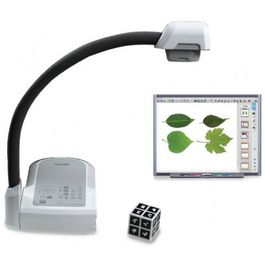
\includegraphics[scale=0.4]{img/pdipedro2.jpg}
\captionof{figure}{Equipo Visualizador Cámara de Documentos}
\end{minipage}
\end{itemize}
 
\item \textbf{Software:}
\begin{itemize}

\item \textbf{INTERWRITE Workspace} : Ofrece una gran cantidad de herramientas que permiten una mayor interactividad en el aula. Incluye reconocimiento de formas, herramientas de edición, etc. Considero que puede ser una herramienta bastante intuitiva. 

\begin{minipage}[hbtp]{1.0\linewidth}
\centering
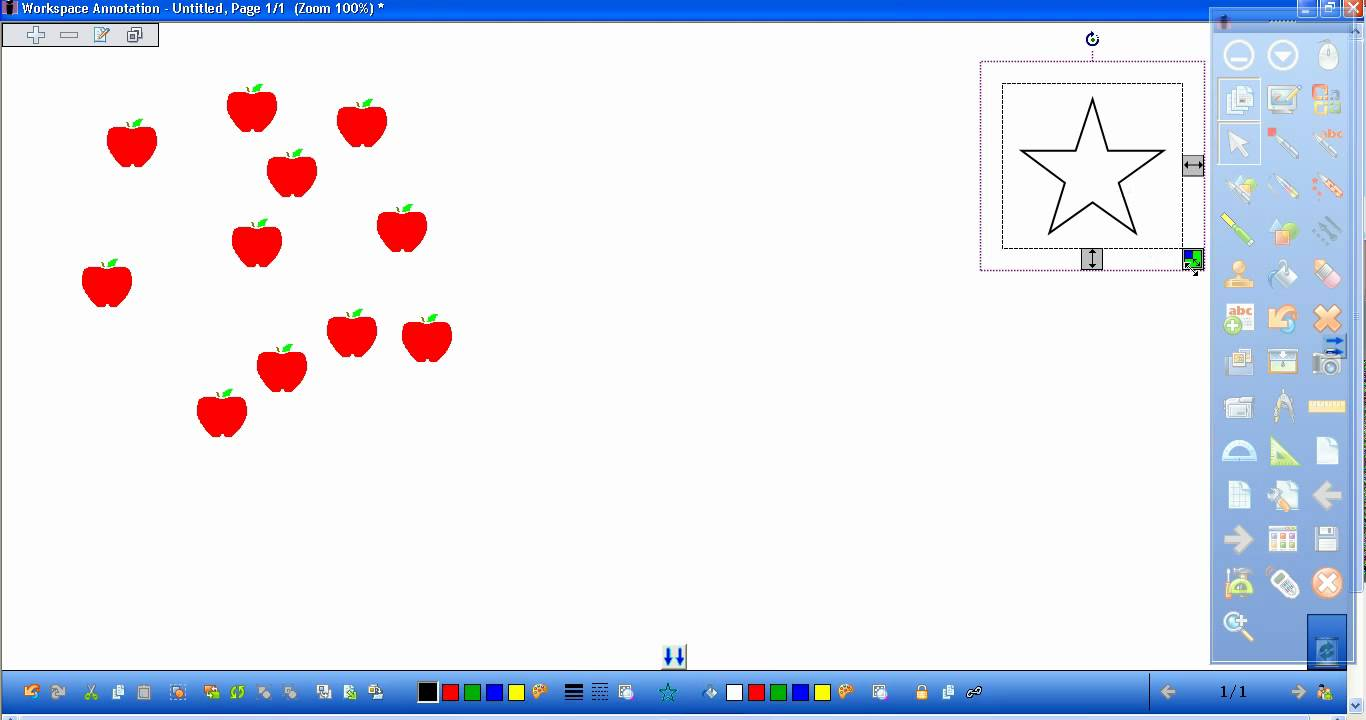
\includegraphics[scale=0.2]{img/pdipedro3.jpg}
%\captionof{figure}{...}
\end{minipage}

 
\item \textbf{Flow} : Permite realizar preguntas improvisadas en clase, y conseguir al instante un conocimiento exacto del nivel de compresión de cada alumno. 
Podemos también crear test y exámenes en cualquier formato (Word, Power-Point, Write, etc ). Dentro de la evaluación en el aula, cabe también destacar Plickers  y Kahoot.
        
\begin{minipage}[hbtp]{1.0\linewidth}
\centering
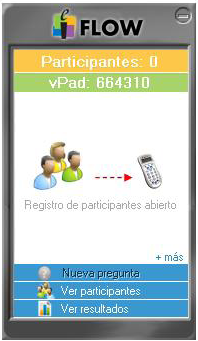
\includegraphics[scale=0.45]{img/pdipedro4.png}
%\captionof{figure}{...}
\end{minipage}

 
\item \textbf{Physics Illustrator} : Este software nos brinda la posibilidad de ver cómo la ley de la gravedad actúa sobre los objetos…un impacto, un desplazamiento, etc. 

 
\begin{minipage}[hbtp]{1.0\linewidth}
\centering
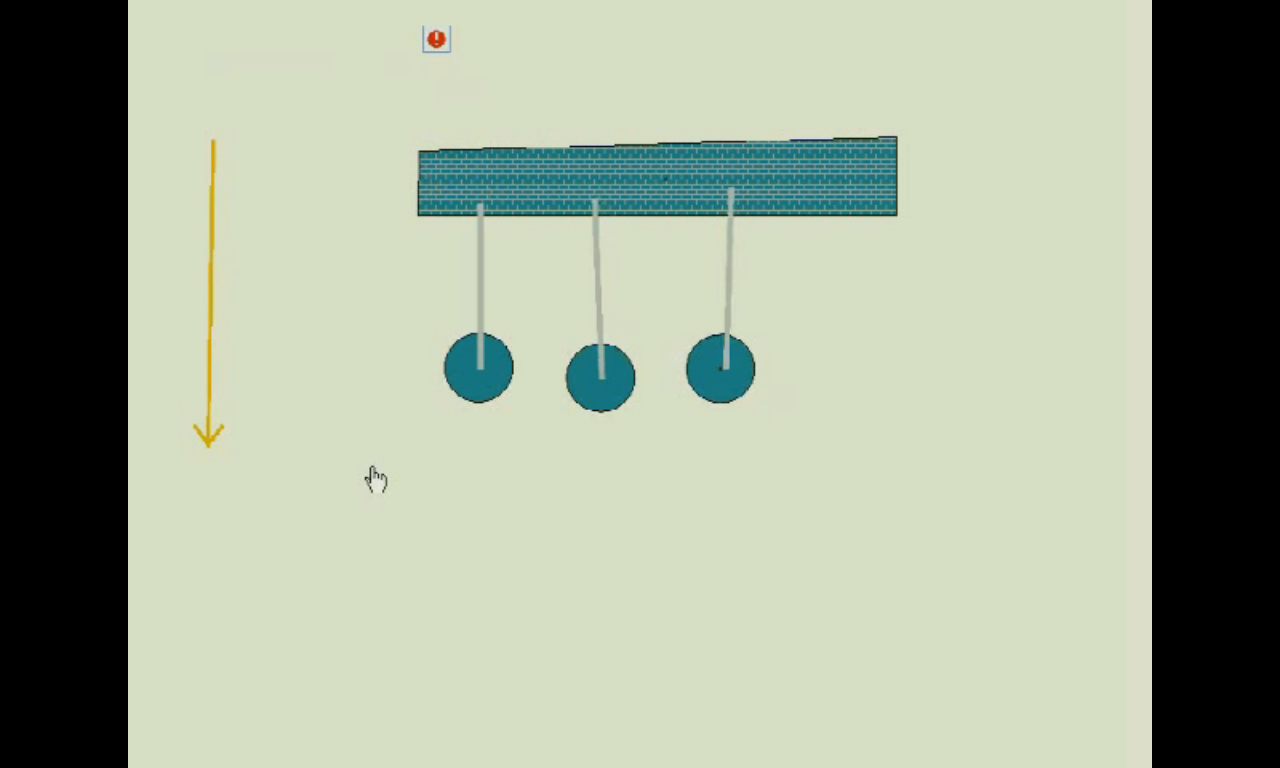
\includegraphics[scale=0.2]{img/pdipedro5.png}
%\captionof{figure}{...}
\end{minipage}

\item Existen otros tipos de software considerados como recursos a la hora de impartir clases, como:  \textbf{easiteach} y \textbf{Graphing Calculator}
 
\end{itemize}
\end{itemize}
\end{opin}

\begin{opin}{\virgicolor}{Virginia}
Este día vino Manuel García Vuelta a darnos una clase muy interesante y productiva sobre los recursos tecnológicos que se puede utilizar en el aula como son las pizarras interactivas. El hecho de ver en directo el propio uso de esos recursos me pareció vital para entender su gran aplicación y la riqueza de este material en el aprendizaje de las distintas asignaturas.

En primer lugar se planteó tres preguntas típicas:

\begin{itemize}

\item Herramientas útiles 

\item Claves del éxito 

\item ¿Cómo puedo formarme? 
\end{itemize}

La respuesta es sencilla: que sean fáciles, adaptables y que sea útiles pedagógicamente.

Asimismo, Manuel nos explicó las distintas etapas para llevar a cabo el uso de estas herramientas en el aula. Con una frase muy sencilla, nos resume la inicial de cada una de ellas: \textbf{Hoy Soy Feliz porque tengo Ayuda:}

\begin{itemize}

\item H, Hardware: se encuentran las pizarras digitales interactivas portátiles o no. Las primeras son más útiles por la comodidad que ofrece la portabilidad. Articlik, que se utiliza para que los alumnos puedan contestar las preguntas del profesor con un mando a través de respuestas opcionales A, B, C o D. También hablo de cámara documentos para enfocar y hacer anotaciones. 

\item S, Software: tiene que ser multiusuario, con formato universal, que sea compatible con todas las pizarras digitales interactivas y que haya licencia para todo el centro. 

\item F, Formación: Hay que realizar un curso presencial motivacional y luego la posibilidad de realizar un curso online para potenciar en cualquier momento lo que se está haciendo. 

\item A, Ayuda: que el profesor pueda contar siempre con ayuda por si le surgiera, por ejemplo, algún problema con el software o el hardware. 
\end{itemize}

Estas fases son muy importantes pero siempre es imprescindible un buen profesor que aproveche bien estos recursos tecnológicos.

Había oído hablar de las pizarras interactivas pero nunca las había visto en funcionamiento, lo cual me pareció fascinante. En todo momento estábamos todos atentos a lo que Manuel nos mostraba, lo cual indica el interés que suscita estos recursos en el aula. Manuel empleó el programa Workspace y junto con otros programas nos enseñó entre otras cosas el movimiento relativo de la Luna con respecto el Sol, y el uso del péndulo. Al ver esto, imaginaba a mi sobrina de 8 años en una clase de este tipo y conociéndola me llamaría contándome lo que había visto en clase y cómo se lo habían enseñado, y desde luego, así no se le olvidaría jamás los conceptos aprendidos ya que los aprende de una forma visual y mediante emociones, y no a base de memorizar o de realizar ejercicios mecánicos que hasta ahora es lo que yo he visto a través de sus deberes.

Otro recurso muy práctico que nos mostró fue cuando se hizo la simulación de un examen y respondimos a las preguntas a través de la aplicación vpad. Creo que sería muy útil incluir por ejemplo al final de cada tema un seguimiento de los conceptos adquiridos por los alumnos realizando un examen tipo test de forma que respondan a través de la aplicación de sus smartphones. Creo que por el hecho de contestar más rápido que sus compañeros o ver quien ha respondido más respuestas correctas a través de la aplicación estarían más motivados en las clases y prestarían más atención para luego realizar este tipo de examen, ya que el usar esta tecnología no lo verían tanto como un examen típico sino incluso como un juego tipo trivial.

Buscando información en internet sobre las pizarras interactivas y sobre Manuel, encontré una presentación interesante del profesor Antonio Solano en el que nos indica que las pizarras se tienen que ver como una ventana al mundo que proyecten y que se utilicen para compartir. Aquí dejo el enlace de la presentación:

 \url{http://es.slideshare.net/ppitufo/pizarra-digital}

Uno de mis problemas a la hora de imaginarme dando clase es ver en las caras de los alumnos su aburrimiento y desmotivación. Desde luego, el uso de estas tecnologías provocaría seguro un cambio de actitud en los alumnos y creo que no hay nada mejor para un profesor que tener alumnos motivados y con ganas de ir a su clase para aprender de una forma diferente y más eficaz. No obstante, y aunque me encantaría que pudiera aplicarse en todas las aulas me temo que con el sistema educativo actual que tenemos hay mucho trabajo por hacer para cambiarlo y conseguir un sistema más progresivo, moderno y que aproveche los recursos tecnológicos.

Desde luego no hay nada como ver en directo a Manuel para motivarte en la educación haciendo uso de las pizarras interactivas, por ello quiero finalizar mostrando este vídeo suyo en el que de nuevo motiva a los profesores al uso de estos recursos tecnológicos:

\url{https://www.youtube.com/watch?v=0x6utJxuw2g}


\end{opin}


\subsection{Innovación y recursos educativos (Tema 3.2 - 14/11/2016)}
\begin{opin}{\guscolor}{Gustavo}

\subsubsection{Recursos educativos en el aula}
Durante la clase de hoy, Raquel nos hizo ver la gran cantidad de recursos didácticos existentes hoy en día en el mundo de las matemáticas. Veo una ventaja muy evidente respecto a buscarlo por nuestra cuenta y es que sin duda Raquel, como docente con años de experiencia, nos ha filtrado los recursos para evitar perdernos en la red.

Esto nos va a ayudar en nuestro futuro profesional como docentes ya que será un espacio dónde poder apoyarnos. Entre otro de los consejos que nos dio Raquel está el de que tenemos que asumir que es difícil estar al día de todo por lo tanto no hay que abrumarse por tal situación.

Los recursos a destacar son:

\subsubsection{Recursos del INTEF}
El Instituto Nacional de Tecnologías Educativas y de Formación  (INTEF) del Profesorado es la unidad del Ministerio de Educación, Cultura y Deporte responsable de la integración de las TIC en las etapas educativas no universitarias. Tiene rango de Subdirección General integrada en la Dirección General de Evaluación y Cooperación Territorial que, a su vez, forma parte de la Secretaría de Estado de Educación, Formación Profesional y Universidades (Fuente: \url{http://educalab.es/intef/introduccion})

Los siguientes recursos se encuentran disponibles desde la web del INTEF \url{http://educalab.es/recursos}, aunque también son interesantes los recursos específicos de matemáticas encontrados en el histórico de recursos \url{http://educalab.es/web/web/recursos/historico/asignaturas/matematicas}

\paragraph{Procomún}
\url{https://procomun.educalab.es/}

PROCOMÚN es el espacio que más destaca dentro de los recursos del INTEF y se describe como una red de Recursos Educativos Abiertos. Este espacio destaca por la gran cantidad de recursos disponibles y por la posibilidad de búsqueda de dichos recursos por medio de los metadatos.

Dentro de Procomún se hizo mención al Proyecto Gauss.

\paragraph{eXeLearning}
\url{http://exelearning.net/}

eXeLearning es una herramienta de autor de código abierto para ayudar a los docentes en la creación y publicación de contenidos web. Facilita la creación de contenidos educativos sin necesidad de ser experto en HTML o XML. Se trata de una aplicación multiplataforma que nos permite la utilización de árboles de contenido, elementos multimedia, actividades interactivas de autoevaluación… facilitando la exportación del contenido generado a múltiples formatos: HTML, SCORM, IMS, etc.

Características destacadas de Exelearning:
\begin{itemize}
\item Permite crear un árbol de navegación básico que facilitará la navegación.  

\item Permite escribir texto y copiarlo desde otras aplicaciones.  

\item Permite incluir imágenes, pero no es un editor de imágenes como Photoshop o Gimp.  

\item Permite incluir sonidos, pero deben estar grabados previamente con otra aplicación.  

\item Permite incluir vídeos y animaciones, pero no permite crearlas.  

\item Permite incluir actividades sencillas: preguntas de tipo test, de verdadero/falso, de espacios en blanco...  

\item Permite embeber elementos multimedia como vídeos, presentaciones, textos o audios.  

\item Permite incluir actividades realizadas con otras aplicaciones 
\end{itemize}


\paragraph{Proyecto Gauss}
\url{http://recursostic.educacion.es/gauss/proc/}

El Proyecto Gauss ha sido desarrollado por el INTEF. Es un proyecto específico de matemáticas y ofrece a los profesores varios centenares de ítems didácticos y de applets de GeoGebra, que cubren todos los contenidos de matemáticas de Primaria y de Secundaria.

\paragraph{Proyecto Agrega/Agrega2}
\url{http://www.agrega2.es/web/}

Este proyecto es una federación de repositorios de contenidos educativos digitales donde todo el mundo pueda buscar, visualizar y descargar material educativo digital no universitario.  Se pretende facilitar a la comunidad educativa una herramienta útil para integrar las Tecnologías de la Información y la Comunicación en el aula

Existe una segunda versión de este proyecto que mejora la anterior y se llama Agrega2. Es de los repositorios más complicados para encontrar cosas. De hecho, hay un curso específico para buscar contenidos en Agrega2.

\paragraph{Red de Buenas PracTICas 2.0}
\url{http://recursostic.educacion.es/buenaspracticas20/web/}

Red de Buenas Practicas 20 es una red social de profesores dentro del INTEF.

\paragraph{Internet en el aula}
\url{http://internetaula.ning.com/}

Otra red social para docentes

\paragraph{Educa con TIC}
\url{http://www.educacontic.es/recursos-educativos}

Es un blog especializado en el uso de las TIC en las aulas

\paragraph{Proyecto Descartes}
\url{http://proyectodescartes.org/}

El Proyecto Descartes comienza su andadura en el año 1998. Lleva mucho tiempo activo, por tanto es lógico pensar que hay mucha documentación y muchos recursos.

Hay una página antigua en una web oficial del ministerio (\url{http://recursostic.educacion.es/descartes/web/}) pero está sin mantenimiento. Esta página antigua lo tenían hecho en JAVA y daba tantos problemas a los usuarios que decidieron cambiarla. Aun así, todavía hay muchos recursos que redirigen de la nueva a la antigua.

La web actual del proyecto Descartes pertenece a la Red Educativa Digital Descartes, que explicamos a continuación.

\paragraph{Red Educativa Digital Descartes}
La Red Educativa Digital Descartes (RED Descartes) es una asociación no gubernamental que se ha constituido el 1 de junio de 2013. Los socios fundadores son profesoras y profesores que tienen una historia conjunta construida, durante quince años, desarrollando proyectos del Ministerio de Educación español, entre los que podemos citar el Proyecto Descartes, Educación Digital a Distancia, Proyecto Canals, Pizarra Interactiva, Newton, Experimentación Didáctica en el Aula, WikididácTICa y Buenas Practicas 2.0. (Fuente: \url{http://www.educacontic.es/blog/matematicas-interactivas-con-descartes-en-tablets-y-smartphones})

En la parte de arriba de la web hay un apartado de subproyectos que te lleva a la página web \url{http://proyectodescartes.org/indexweb.php} . Entre estos subproyectos destacan:
\begin{itemize}
\item Telesecundaria (\url{http://proyectodescartes.org/Telesecundaria/}): educación a través de videos. Ojeando esta aplicación, también hay ejercicios y explicaciones interactivas hechas con HTML5, lo cual hace que sea accesible a través de cualquier navegador moderno. 

Telesecundaria es además una modalidad en el sistema educativo de México.

 

\item Proyecto Canals (\url{http://proyectodescartes.org/canals/index.htm}) de la profesora catalana Maria Antònia Canals para infantil y primaria. 

 

\item Proyecto "EDAD" Educación Digital con Descartes (\url{http://proyectodescartes.org/EDAD/index.htm}) surge con el propósito de desarrollar recursos educativos digitales interactivos, para la Educación Secundaria Obligatoria (ESO) en las áreas curriculares de Matemáticas, Ciencias Naturales y Física y Química, que permitan su uso tanto en la enseñanza presencial como en la formación a distancia. 

 

\item Proyecto ASIPISA (\url{http://proyectodescartes.org/ASIPISA/index.htm}). ASIPISA es una palabra palíndroma, acrónimo de “Ayuda Sistemática Interactiva para PISA”, que da nombre a un proyecto de desarrollo de materiales educativos, digitales e interactivos, basados en las unidades liberadas del Programa internacional PISA 

 

\item Proyecto Competencias (\url{http://proyectodescartes.org/competencias/index.htm}): Pensado para formar en competencias como marcan los nuevos planes de estudios. Esta web recoge objetos de aprendizaje interactivos cuyo objetivo es la formación y evaluación competencial. Sus contenidos se basan en las unidades liberadas de PISA, en las de las Pruebas de Evaluación de Diagnóstico de diferentes Comunidades autónomas españolas de acuerdo a la Ley Orgánica de Educación (LOE) de 2006 y a las pruebas de Evaluación de diagnóstico establecidas por la Ley Orgánica para la Mejora de la Calidad Educativa (LOMCE) de 2013. 
\end{itemize}

\paragraph{Educarex}
Es el Portal con contenidos educativos de la Comunidad Extremadura. Extremadura estaba a la cola en educación e hizo un esfuerzo bestial para ponerse a la altura del resto de España. Este portal es parte del fruto de dichos esfuerzos.

\paragraph{Otros recursos}
Además de todo lo visto hasta ahora también existen otros recursos como revistas, blogs, páginas de internet, etc. A continuación se citan algunos de estos recursos para su conocimiento:
\begin{itemize}
\item Aulaplaneta es un sistema integrado de contenidos curriculares que pone al servicio del profesor una propuesta didáctica personalizable y gran variedad de recursos digitales para preparar sus clases, y a disposición de los alumnos todo lo que necesitan para aprender de forma motivadora y eficaz. Destacar el artículo ” Diez canales educativos imprescindibles de YouTube para alumnos y profesores” \url{http://www.aulaplaneta.com/2015/10/27/recursos-tic/diez-canales-educativos-imprescindibles-de-youtube-para-alumnos-y-profesores/}  

 

\item MisMates y TutorMates. Se trata de dos proyectos digitales de Oxford destinados para el área de Matemáticas.   

MisMates es una aplicación educativa de acceso exclusivamente on line y está enfocada al alumnado de entre 1º y 4º de la ESO que tiene a su disposición varias áreas de trabajo, un editor de expresiones matemáticas y una libreta digital.

TutorMates es una aplicación de escritorio para Windows, iOS o Linux, y trabaja con herramientas específicas los contenidos de cada bloque

 

\item Educacion 3.0 es una revista de elevado interés en el mundo educativo en el que destaca el artículo “15 recursos de Internet imprescindibles para cualquier profesor” \url{http://www.educaciontrespuntocero.com/recursos/recursos-para-educacion-profesor-imprescindibles/35931.html}  

 

\item ScolarTIC es un proyecto de la Fundación Telefónica. Es una Comunidad Educativa de ámbito hispano. Es un espacio social de aprendizaje, innovación y calidad educativa en el que se ofrecen cursos online gratis, recursos para el aula así como charlas, ponencias y talleres.  

 

\item Y además a nivel particular hay muchas webs de profesores que ponen su trabajo al servicio de los demás: 
\begin{itemize}
\item Pilarleku@ (\url{http://pilarlekunew.blogspot.com.es/}) 

\item Domingo Mendez \url{http://domingomendez.es/} y su blog “Educación y TIC” \url{http://domingomendez.blogspot.com.es/}  

\item Algebra con Papas \url{https://www.edu.xunta.es/espazoAbalar/sites/espazoAbalar/files/datos/1291360755/contido/index.htm}  

\item Thatquiz \url{https://www.thatquiz.org/es/} Web con cuestionarios de matemáticas 

\item Manuel Sada Allo y su web Ejemplos diversos de webs interactivas de Matemáticas \url{http://docentes.educacion.navarra.es/msadaall/geogebra/}  

\item Sectormatematica \url{http://www.sectormatematica.cl/}  

\item Antonio Perez Sanz \url{http://platea.pntic.mec.es/}~aperez4/. Antonio presentó los programas de TVE de “Más por menos” y “Universo Matemático”. Actualmente (Diciembre de 2016) es responsable de divulgamat. 

\item “Amo las mates” actualmente en la web \url{https://www.matematicasonline.es/}  

\item Disfruta las matemáticas \url{http://www.disfrutalasmatematicas.com/}  

\item Vitutor \url{http://www.vitutor.com/} también se usa para la universidad. Tiene un contenido de bachillerato bastante potente. es una plataforma de teleformación diseñada para el aprendizaje en línea de distintas materias. 

El proyecto comenzó con la especialización en contenidos de Matemáticas, y estamos trabajando en otras materias, como inglés.

\item  “Aula21” que en su página \url{http://www.aula21.net/primera/matematicas.htm}  recopila un listado de enlaces a recursos de interés en el mundo de las matemáticas. 

\item Banco de recursos de SM \url{http://www.smconectados.com/Banco_de_recursos.html} donde encontrarás recursos para ayudarte a hacer más fácil tu trabajo en el aula. 
\end{itemize}
\end{itemize}

\paragraph{9 cosas que los profesores digitalmente competentes hacen habitualmente}


\begin{minipage}[h]{1\linewidth}
	\centering
	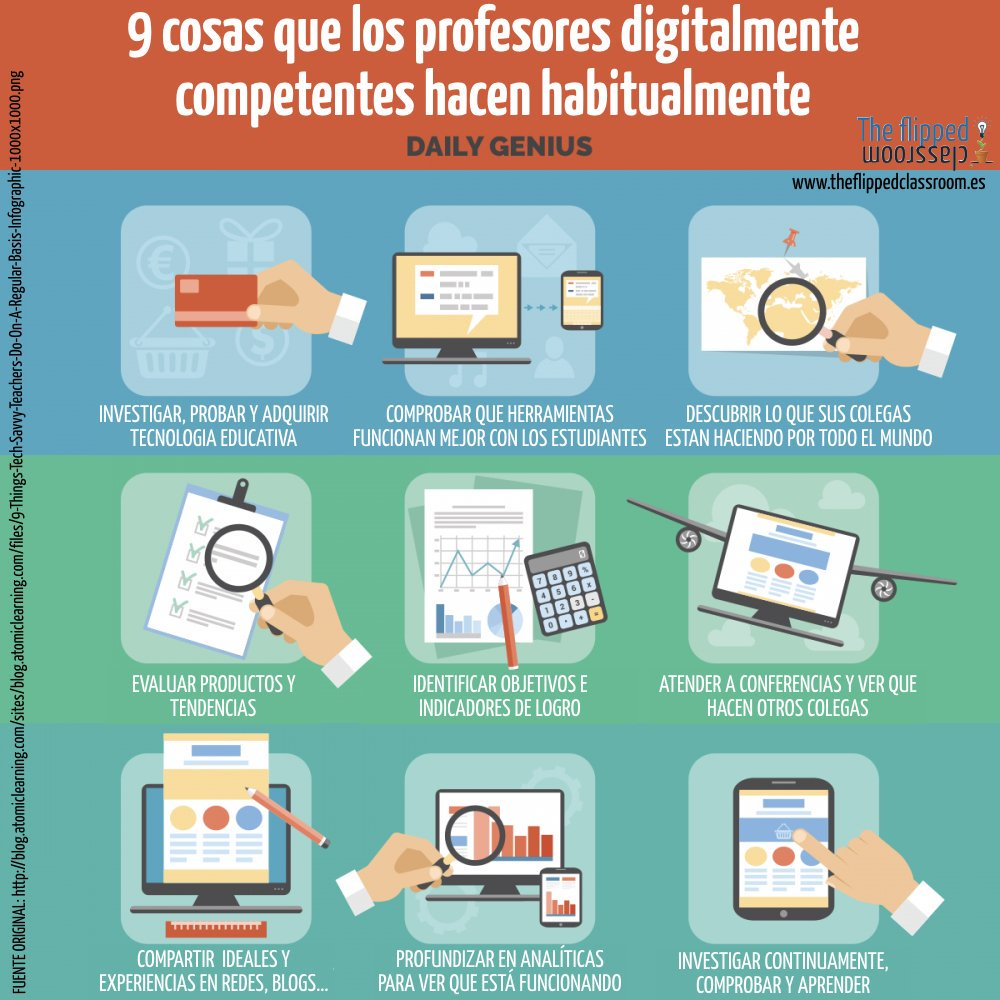
\includegraphics[width=0.8\linewidth]{img/9cosasdegus.jpg}
	\captionof{figure}{Coche de mediadios del siglo pasado.}
\end{minipage}

 
\paragraph{Uso del video en educación}
No cabe duda que el uso del video en la clase es una metodología innovadora. Está claro que tiene muchas ventajas como por ejemplo la de romper con la monotonía de la clase, pero también puede haber inconvenientes.

Los tipos de videos educativos según \url{http://www.uclm.es/profesorado/ricardo/Video/2002_2003/sld003.htm} son:

\begin{itemize}
\item \textbf{Documentales:} muestran de manera ordenada información sobre un tema concreto. 

\item \textbf{Narrativos:} tienen una trama narrativa a través de la cual se van presentando las informaciones relevantes para los estudiantes.  

\item \textbf{Lección monoconceptual:} son vídeos de muy corta duración que se centran en presentar un concepto.  

\item \textbf{Lección temática:} son los clásicos vídeos didácticos que van presentando de manera sistemática y con una profundidad adecuada a los destinatarios los distintos apartados de un tema concreto .  

\item \textbf{Vídeos motivadores:} pretenden ante todo impactar, motivar, interesar a los espectadores, aunque para ello tengan que sacrificar la presentación sistemática de los contenidos y un cierto grado de rigor científico. 
\end{itemize}

Un video motivador para poner a los alumnos puede ser el video de Tadeo Jones \url{http://www.telecinco.es/tadeojones/descubre-con-tadeo/Tadeo_Jones-Descubre_con_Tadeo-Matematicas_2_1697355179.html}

Otro video que impresiona a la hora de demostrar como la perspectiva puede engañar a como nuestro ojo le pasa la información a nuestro cerebro es \url{https://www.youtube.com/watch?v=U9PZizBDBZw} en el que colocando una serie de velas en un suelo plano y la posición de la cámara el autor nos muestra como da la sensación de que se acaba formando un cubo en 3 dimensiones sobre el que es capaz de sentarse.

Otro video fascinante es el de las potencias de 10 \url{https://www.youtube.com/watch?v=fbCwkfrKuaw} en el que nos muestran un “zoom out” con 10 elevado a n veces para salir al espacio y un “zoom in” con $\rfrac{1}{10}^n$ para adentrarnos en el organismo de las personas. El zoom out es otra manera de explicar los Sistemas de Información Geográfica como puede ser el de Google Maps.

Recursos de videos educativos pueden ser:
\begin{itemize}
\item El canal derivando de Youtube que son videos de Eduardo Sáenz de Cabezón \url{https://www.youtube.com/channel/UCH-Z8ya93m7_RD02WsCSZYA} 

\item “La pizarra de Fonemato” (www.matematicasbachiller.com) que contiene videos explicativos con una característica muy peculiar y es que lo explica todo muy despacio con un tono de voz serio que a la vez puede resultar cómico. 

\item El portal MatematicasIES \url{http://matematicasies.com} creado por Daniel López Avellaneda, Licenciado en Ciencias Matemáticas por la Universidad de Granada y Profesor de Matemáticas y Coordinador TIC en el IES Mar Serena. 

\item El portal Educacion 3.0 visto anterormente tiene recursos para crear videos como profesores. \url{http://www.educaciontrespuntocero.com/experiencias/recursos-para-grabar-lecciones-en-video/33017.html}  

\item Unicoos que es un portal de videos gratuitos para las asignaturas de ciencias. Enfocado a estudiantes de Secundaria, Bachillerato y universitarios.  

El portal Unicoos de YouTube proporciona algo más de 600 vídeos gratuitos para las asignaturas de Matemáticas, Física y Química. \url{https://www.youtube.com/user/davidcpv}
\end{itemize}

\paragraph{Matemáticas recreativas}
“La matemática recreativa se concentra en la obtención de resultados con actividades lúdicas, y a difundir o divulgar de manera entretenida y divertida los conocimientos o ideas o problemas matemáticos. Es un concepto tan viejo como lo son los juegos en los que interviene la lógica o de algún modo el cálculo” (Fuente: Wikipedia)

Es importante que los alumnos lleguen a ver que todos los juegos tienen una explicación matemática detrás. Llegar a sorprenderles es algo que logra captar su atención. Si recordamos en la página www.divulgamat.net hay una sección llamada Sorpresas Matemáticas en la que podremos encontrar bajo el menú principal recursos de este tipo


 
Un video que \textbf{llega a sorprender} a los alumnos es el de “crear chocolate de la nada” \url{https://www.youtube.com/watch?v=Y13tSEyOqGs.} En el video se consigue partir el chocolate y luego volver a reconstruir dando la sensación de que sobra una onza de chocolate. En realidad no se crea chocolate, es un truco creado que trabaja con diferentes pendientes de la recta que son cercanas y se puede manipular para aparentar que vuelve a su estado natural cuando no es cierto. La explicación detallada está en este otro video \url{https://www.youtube.com/watch?v=eb2hCmc2xso}

 

\paragraph{Anamorfismo y futbol\\}
 

\begin{minipage}[h]{1\linewidth}
	\centering
	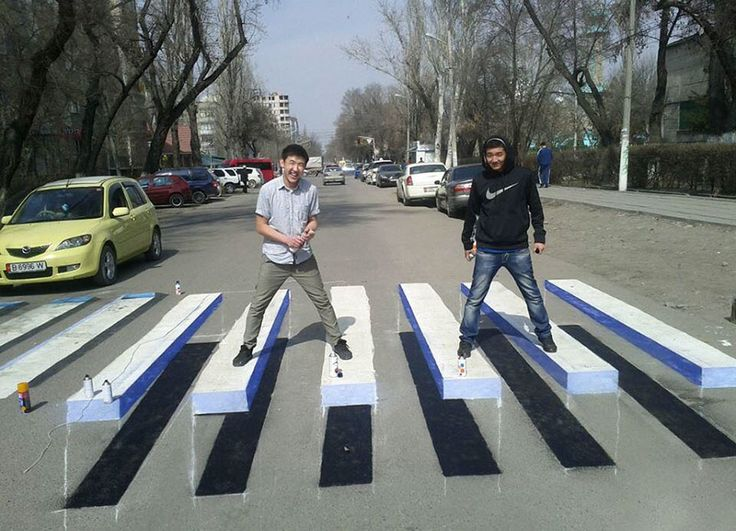
\includegraphics[width=0.7\linewidth]{img/anamorf1.jpg}
\end{minipage}
 
Otro ejemplo de matemáticas recreativas es el del anamorfismo. Consiste en deformar la imagen a través de efectos ópticos o a través de un procedimiento matemático con perspectivas. Uno de los artistas más destacados utilizando esta técnica es Julian Beever. “Julian es un artista británico que se dedica a dibujar con tiza. Ha creado dibujos de tiza en 3D en el pavimento utilizando un método llamado anamorfosis que crea una ilusión óptica. Sus dibujos en las calles desafían las leyes de la perspectiva. Ha logrado una técnica que le da un gran realismo a la imagen” (Fuente: Wikipedia).

\begin{minipage}[h]{1\linewidth}
	\centering
	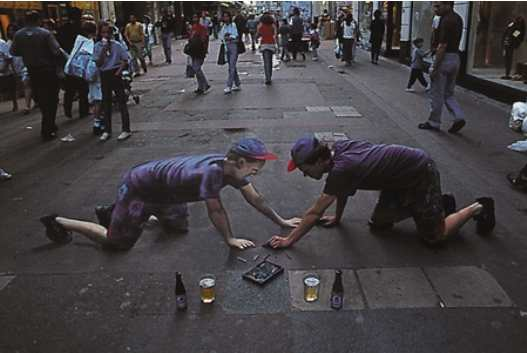
\includegraphics[width=0.7\linewidth]{img/anamorf2.jpg}
	
\end{minipage}
 
Un ejemplo de anaformismo de un cubo de Rubik en video se puede ver en  \url{https://www.youtube.com/watch?v=ooY7Mf0JlNM.} En este video nos permiten incluso acceder a la imagen que permite hace dicho anaformismo. Se puede descargar de \url{https://docs.google.com/file/d/0B3gyYFZJgwKVZ24zWDV1VVB5Wms/edit.} De hecho, me he descargado la imagen.

\begin{minipage}[h]{1\linewidth}
	\centering
	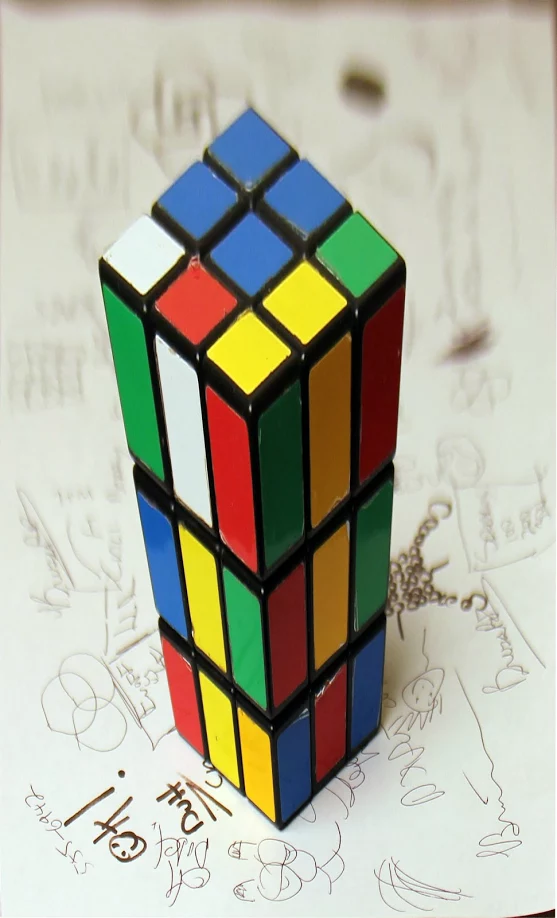
\includegraphics[width=0.7\linewidth]{img/anamorf3.png}
\end{minipage}
 
Por último, nos preguntaremos que tiene que ver el futbol con el anamorfismo. Pues bien, una vez visto que a la técnica que permite crear esta ilusión óptica se le llama anamorfismo, decir que en el futbol, principalmente en los partidos de primera división aprovechando el angulo de proyección de la grabación de las cámaras de televisión “colocan” la publicidad pintada en el plano para producir un efecto en 3D.

\begin{minipage}[h]{1\linewidth}
	\centering
	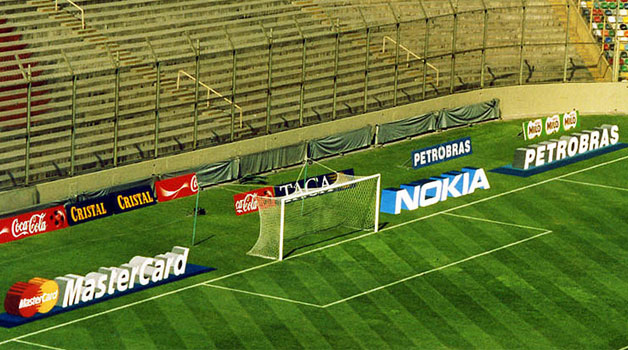
\includegraphics[width=0.7\linewidth]{img/anamorf4.jpg}
\end{minipage}
 
\paragraph{El cine y la literatura como recursos didacticos}
Por último, hay una gran cantidad de literatura matemática. No por ser matemáticos debemos olvidar la literatura. De hecho la convivencia entre ambas es fundamental.

Los siguientes enlaces tienen un montón de recursos literarios matemáticos:
\begin{itemize}
\item \url{http://aulamatematica.com/libros/libros_recomendados.htm}  

\item \url{http://www.librosmaravillosos.com/} en el que hay un buscador de libros gratuitos de difusión científica. 
\end{itemize}
El cine también ha servido como fuente de inspiración para muchos directores y guionistas a la hora de difundir las matemáticas:
\begin{itemize}
\item Una mente maravillosa 

\item El código Da Vinci 

\item Black Jack 

\item La vida es bella 

\item Cube 

\item Agora 

\item Contact 

\item Blade Runner 

\item El día de la bestia 

\item Moebius 

\item 3:19 

\item Granujas de medio pelo 
\end{itemize}
O como el caso de la “Jungla de Cristal 2” donde los protagonistas tienen que resolver el problema de las garrafas de 3 y 5 galones de agua. Para desactivar la bomba tienen que conseguir 4 galones exactos en una de las garrafas. ¿Cómo lo conseguirán? Aunque en la película no se explica claramente, se consigue (Fuente: \url{http://www.sociedadmatematicacantabria.es/Probl_Olimpiada/Sol_probl_3_2.htm}):
\begin{itemize}
\item 1º Llenas la de 5 y echas lo que puedas en la de tres.  

Quedan 3L en la de 3 y 2L en la de 5

\item 2º Vacías la de 3 y echas los 2L de la de 5 en la de 3.  

Quedan: 2L en la de 3 y 0L en la de 5

\item 3º LLenas la de 5 y echas lo que puedas en la de tres (1L)  

Quedan: 3L en la de 3 y 4L en la de 5

\item 4º Vacías la de 3 y ya tienes 4L en la de 5 
\end{itemize}

\paragraph{Khan Academy \url{https://es.khanacademy.org}}
Por último, no quería dejar sin mencionar en el portafolios la aportación realizada en el foro  por mi compañero de grupo Victor De Juan sobre la “Khan Academy”.

Khan Academy es una web que ofrece ejercicios de práctica, videos instructivos y un panel de aprendizaje personalizado que permite a los alumnos aprender a su propio ritmo, dentro y fuera del salón de clases. Y todo ello sin pagar ni un duro.

En este video de la Universidad Politécnica de Valencia nos explican cómo comenzar a usar esta web tanto si somos alumnos, profesores o padres. \url{https://www.youtube.com/watch?v=FvacPlqEw6g}

 


\end{opin}

\begin{opin}{\victorcolor}{Víctor}

Hoy ha sido un bombardeo de recursos para utilizar en clase. Paginas web, blogs, educalab... 
%
A día de hoy se me queda lejano porque no he profundizado sobre los recursos. 
%
Parece que voy a tener que estudiarme y bucear por todos estos recursos para descubrir cuáles me gustan más, cuáles me parece que pueden ser más útiles, etc.
%
La cantidad de tiempo invertido en filtrar 


\subsubsection{Ideas interesantes}

\begin{itemize}
	\item ¿Porqué no, hablar todos los años de quién ha ganado la medalla Fields?
\end{itemize}

\end{opin}

\begin{opin}{\pedrocolor}{Pedro}

.


\end{opin}

\begin{opin}{\virgicolor}{Virginia}
.


\end{opin}



\section{Conclusiones de la asignatura}


\subsection{Conclusiones de Gustavo}
\begin{leftbar}{\guscolor}
\subsubsection{Valoración de la asignatura}

Quería realizar una valoración de la asignatura sin revisar el primer apartado que hice a principios de curso sobre las expectativas de la asignatura. De esta manera podré comprobar fielmente las diferencias entre lo que esperaba al empezar la asignatura y lo que he valorado al terminar la misma.

Durante la asignatura he aprendido muchas cosas, pero si tuviese que reflejar de manera clara y concisa las conclusiones principales que saco son:

\begin{itemize}
\item El aprendizaje va de la mano de las emociones y de la motivación.
\item Hay un nuevo campo reciente que está por investigar: la neurociencia.
\item Hay que buscar metodologías de enseñanza diferentes a la tradicional.
\end{itemize}

Existen infinidad de recursos para los docentes

En relación al número de horas de impartición de la asignatura he de decir que el tiempo de horas impartidas de clase a la asignatura no es tan elevado como debería para los contenidos que se pretenden. En total hemos tenido 9 días de clase de 2 horas. 18 horas de clase de las cuales 4 clases han sido “clases magistrales” impartidas por Raquel, 1 clase de pizarras digitales impartida por Manuel y 4 clases de exposición de trabajos.

10/10/2016 Clase 01. T01. Innovación en Educación

17/10/2016 Clase 02. T02. Introducción a la Neurodidáctica

24/10/2016 Clase 03. T02. Introducción a la Neurodidáctica

24/10/2016 Clase 03. T03. Innovación y recursos educativos

07/11/2016 Clase 04. Clase magistral de Pizarras digitales

14/11/2016 Clase 05. T03. Innovación y recursos educativos

21/11/2016 Clase 06. Exposición de trabajos Dia 1

28/11/2016 Clase 07. Exposición de trabajos Dia 2

05/12/2016 Clase 08. Exposición de trabajos Dia 3

12/12/2016 Clase 09. Exposición de trabajos Dia 4

A pesar de que este número de horas no es elevado, reconozco que el hecho de tener que trabajar el portafolio hace que las horas dedicadas a la asignatura aumenten considerablemente. Esta dedicación nos permite profundizar en los contenidos vistos en clase y es de aquí de donde saco la conclusión más importante y es que esta asignatura en general y el portafolio en particular es una herramienta muy útil para nuestro futuro como profesores de matemáticas.

También he de reconocer que me gustaron más las primeras clases de la asignatura por lo novedoso pero con el paso del tiempo, no sé si por rutina o porque realmente las clases fueron cambiando, me resultaron más tediosas. Las primeras clases fueron más colaborativas con preguntas y debates promovidos por los alumnos y comentados con la profesora. Este tipo de clases me resultan mucho más atractivas, pero es cierto que es una opinión muy personal. Sin embargo, el hecho de que tuviésemos tan pocas horas disponibles, las clases fueron tornando y me dio la sensación de que se limitaban a indicar enlaces a recursos didácticos en el mundo de las matemáticas. Reconozco que nos va a ser muy útil en el futuro tener acceso a estos recursos, pero la utilidad real la obtendremos cuando seamos docentes y tengamos que hacer uso de estos recursos. A día de hoy no le podemos sacar el 100\% del jugo a la asignatura.

Por ser constructivo lo que yo haría en el futuro sería un par de cambios. El primero puede parecer un poco drástico. Sería eliminar los trabajos y las exposiciones con el objetivo de ganar horas de clase. Quizá al tener más tiempo se resolvería el segundo cambio que es el de que las clases fuesen más colaborativas. Generar debates y conocer la opinión de todos los alumnos sobre los distintos temas tratados en clase nos enriquecería mucho más al aplicar en clase lo aprendido (trabajo colaborativo). Esto es una conclusión y una evidencia que he aprendido de la propia asignatura así que, ¿por qué no emplearlo para nuestra propia clase?

Como no todo son cambios, para terminar mis valoraciones, yo mantendría el portafolio porque como ya he comentad, es una buena manera de repasar los conceptos vistos en clase.

Y llegados a este punto, acabo de leer cuales eran mis expectativas iniciales. La diferencia más clara entre las conclusiones que he sacado y las expectativas iniciales han sido que inicialmente esperaba que se hubiese hecho más hincapié en las TICs y sin embargo las TICs no han eclipsado a todo lo que hemos aprendido.

\subsubsection{Valoración de mis compañeros}
Con respecto a mis compañeros, pues qué voy a decir de ellos. Que me parecen unos excelentes estudiantes y sobre todo unas bellísimas personas. Solo tengo buenas palabras para ellos.

Han hecho una labor de equipo excelente durante todo el curso. Como valoración global de los 3 les pondría un sobresaliente sin dudarlo.

\subsubsection{Autoevaluación}

\end{leftbar}

\subsection{Conclusiones de Víctor}
\begin{leftbar}{\victorcolor}

\subsubsection{Valoración de la asignatura}

En esta asignatura, más que quedarme con los contenidos concretos, me quedo con la motivación recibida.
%
Esta asignatura (debido a la motivación intrínseca de la profesora) me ha ayudado a tomar conciencia de la importancia que tendrá mi labor. 
%
Antes de entrar ya era consciente que las Matemáticas son la asignatura difícil con la que algunos se atragantan, pero no era consciente de la magnitud del problema que eso supone.

A día 11 de Diciembre, si tengo que resumir la asignatura en una palabra sería \textbf{Motivación}. 
%
Termino la asignatura muy motivado con la labor que me espera, con más ganas de empezar las prácticas y con una idea muy clara de que eso de 2 meses de vacaciones es mentira, porque tengo tantísimos recursos que consultar, tantas posibilidades con las que innovar, que, como poco, la mitad de cada verano lo acabaré invirtiendo en cómo innovar y mejorar mi labor docente.

Me llevo también el ejemplo de que desde la Universidad, aunque este máster se considere un trámite, existen profesores muy motivados que viven su trabajo muy vocacionalmente. 
%
He disfrutado mucho de la docencia impartida desde el convencimiento de que sirve para mucho, de que el cambio necesario en la educación empieza por formar a los profesores con un máster de verdad y no un mero trámite. Si alguna vez acabo formando a futuros docentes (que nunca me lo había planteado hasta ahora), será gracias a esta asignatura en primer lugar, más por la profesora que por la asignatura en sí. 

\subsubsection{Valoración de mis compañeros}

El grupo de trabajo lo escogimos por comodidad, ya que éramos el mismo grupo en otra asignatura (Didáctica de las Matemáticas).
%
Como grupo hemos funcionado muy bien, creo que hemos sido muy comprensivos y hemos sabido trabajar en equipo.
%
Estoy muy gratamente sorprendido de lo bien que hemos trabajado. Haber formado los grupos por cómo estábamos sentados en otra asignatura ha dado muy buen resultado.

Mis compañeros son muy responsables, eficientes y trabajadores y estas dinámicas tan positivas me han animado a ser todavía más trabajador, eficiente y responsable de lo que era anteriormente. 
%
Hemos sabido aportar todos lo que era necesario y no ha hecho falta nunca llamar la atención a nadie por nada.

Por último, valoro muy positivamente los conocimientos previos de cada uno. Venir de carreras diferentes ha sido muy positivo, tanto para el ámbito profesional (del trabajo de la asignatura) como para el ámbito personal (de conocer personas con otras historias y entornos diferentes).

\subsubsection{Autoevaluación}

Como todo en esta vida, siempre se puede hacer mejor y siempre hay margen de mejora. 
%
Dicho esto, creo que he trabajado bastante bien. 
%
Sólo no he podido ir a una clase y en clase siempre he mantenido la concentración en lo que se estaba tratando.
%
La mayor dificultad ha sido saber priorizar lo importante sobre lo urgente. 
%
Debido al resto de mis responsabilidades (voluntariado, cursos y otros estudios) siempre tenía algo más urgente que hacer que revisar con profundida los recursos.
%
No obstante, creo que durante mi práctica laboral podré sacarle todo el jugo a los recursos facilitados por la profesora.
%
Eso sí, como las jornadas complementarias sólo ocurren una vez, y a los recursos puedo acceder en otro momento, he intentado ir a todas las jornadas complementarias (aunque no me ha sido posible ir a todas).

\end{leftbar}

\subsection{Conclusiones de Pedro}
\begin{leftbar}{\pedrocolor}

\subsubsection{Valoración de la asignatura}

La asignatura me ha permitido aprender numerosos conceptos, metodologías y recursos educativos que desconocía anteriormente. Es indudable su gran aporte a mi formación como profesor. Me gustaría con el tiempo ir poco a poco analizando en profundidad cada una de las aportaciones realizadas en cada sesión, con la finalidad de potenciar al máximo su efectividad en el aula. 

El trabajo grupal me ha permitido tomar conciencia de lo importante que es saber organizarse, cooperar y escuchar las sugerencias del resto de compañeros. He aprendido mucho de sus aportaciones, vivencias educativas y sus puntos de vista como futuros educadores.

Para finalizar, y no por ello menos importante, destacar la gran importancia de las Jornadas de Formación Complementaria. Me han acercado a las metodologías activas y a las teorías y ciencias en las que se basan. Espero haber adquirido las herramientas necesarias para trabajar en el aula con mis futuros alumnos. 

Llegué al máster pensando que el mejor profesor era el que más sabía, pero como dijo Irene Ros en su Jornada, “No es mejor profesor quien más sabe, sino quien más consigue que aprendan sus alumnos”.

\subsubsection{Valoración de mis compañeros}

Mis compañeros de grupo han respondido muy bien a la hora de realizar las actividades. Pese a tener todos responsabilidades fuera del Máster, en ningún momento han mostrado signos de flaqueza para sacar el trabajo adelante. A la hora de proponer una temática para el trabajo final, me ha sorprendido la gran capacidad creativa que tienen y la profesionalidad con la que tratan los temas.

\subsubsection{Autoevaluación}

Me he sentido como en “Howarts”, escuela a la cual asisten jóvenes matemáticos e ingenieros para desarrollar sus habilidades mágicas como educadores.  Eso ha sido para mí esta asignatura, dar nombre y definición a los problemas que vengo observando toda la vida como alumno y que ahora tengo la obligación como docente, de buscar solución para sacar lo mejor de cada alumno. 

\end{leftbar}

\subsection{Conclusiones de Virginia}
\begin{leftbar}{\virgicolor}


\subsubsection{Valoración de la asignatura}
Esta asignatura ha cumplido con creces mis expectativas iniciales al mostrarme nuevos métodos de aprendizaje aplicando técnicas como la neurodidáctica, y haciendo uso de múltiples recursos tecnológicos aportándome una información muy valiosa para mi futura carrera como profesional docente.

Mi visión como profesora ha dado un vuelco, ahora me siento más motivada y con ganas de hacer cosas nuevas, me ha animado a ser partícipe en la transmisión de conocimientos de una forma diferente a la típica clase magistral de forma que ahora el alumno sea un agente activo en lugar de pasivo, se trabaje de forma colaborativa en clase promoviendo el aprendizaje social y se haga uso de forma adecuada de la multitud de recursos tecnológicos que existen.

No obstante es una ardua tarea ya que en primer lugar el sistema educativo actual tiene que mejorar mucho para facilitar los nuevos métodos de aprendizajes. Así mismo, y dado toda la información y recursos de los que dispone el docente, es muy importante realizar cursos de formación del uso de los nuevos métodos y las nuevas tecnologías para realizar un buen uso de ello y conseguir así un aprendizaje permanente.

En cuanto al trabajo en grupo me ha parecido muy útil y divertido ya que he vivido en primera persona lo que es el trabajo colaborativo aprendiendo cosas de mis compañeros e intentando aportarles a ellos de igual forma otras cosas.

Para finalizar me quedo con la frase que dijo José Ramón Gamo en una de sus charlas: “el cerebro aprende emocionándose”. Por tanto, la labor del docente tiene que ser conseguir con su enseñanza emocionar a los alumnos de forma que estén más motivados y con ganas de más.

\subsubsection{Valoración de mis compañeros}


Con respecto a mis compañeros de trabajo, estoy muy contenta de haber trabajado con ellos ya que creo que nos hemos entendido muy bien y hemos trabajado a gusto.
%
El hecho de proceder de carreras diferentes creo que ha sido muy útil a la hora de aportarnos cosas diferentes.
%
 Además, en algún momento de agobio por la carga de trabajo que se nos presentaba me he sentido apoyada y aliviada por las palabras de mis compañeros.
%
En definitiva, son trabajadores, responsables y buenos compañeros, por lo que estoy muy contenta de haber formado parte de este grupo.



\subsubsection{Autoevaluación}
En general ceo que mi trabajo en esta asignatura ha sido bastante bueno ya que he asistido regularmente, salvo el último día que por motivos de trabajo y personales no pude.
%
Además, he intentado llevar al día el portafolio para facilitar un transcurso continuo de la asignatura lo que me ha permitido trabajar más cómoda y sin prisas.
%


Por otro lado, mi principal problema tanto en esta asignatura como en el resto ha sido la falta de tiempo ya que trabajo a jornada completa además de realizar también un curso de inglés.
%
Por tanto, no he podido dedicar todo el tiempo que hubiera querido a revisar toda la información complementaria que Raquel nos ha aportado y por desgracia tampoco he podido asistir a las jornadas complementarias que tanto me hubiera gustado, sobre todo, la de Javier Blumenfeld y José Ramón Gamo.
%
No obstante, gracias a Internet he podido asistir virtualmente a alguna charla de ellos.
%
Además, soy consciente de la multitud de recursos de los que disponemos, entre otros, toda la información complementaria que Raquel nos ha aportado y de los que iré haciendo uso durante el transcurso del máster y durante mi futuro profesional como docente ya que creo que es una información muy valiosa para conseguir que mis futuros alumnos se emocionen mientras aprendan.


\end{leftbar}



\chapter{Trabajo de Innovación educativa}


Este trabajo ha sido realizado por \theauthor y está dirigido a 1 de Bachillerato del itinerario de Ciencias Sociales.
%
No trata una unidad didáctica específica, sino que se enfoca a la presentación de la asignatura el primer día de clase.


\section{Introducción}


\subsection{Elección y Justificación}

Matemáticas es una asignatura que a bastante porcentaje del alumnado se le hace difícil. 
%
Hay algunos que optan por otros itinerarios sólo para evitar las Matemáticas, porque ya les parecen imposibles.
%
Hay otros que eligen Matemáticas "fáciles" (Matemáticas aplicadas a las Ciencias Sociales) porque no quieren ni Física ni Latín.

Sin saber con seguridad qué porcentaje del alumnado de esas "Matemáticas fáciles" la ha escogido por gusto o por ser la opción \textit{menos mala}, creemos que a un alto porcentaje del alumnado de 1 de Bachillerato de Sociales no le gustan las Matemáticas y que, además, pueden pensar que se les da realmente mal. 
%
Es por ello que queríamos hacer el trabajo para, de alguna manera, solucionar este problema que creemos que se da en el Bachillerato de Sociales.

Aunque una consigna de este trabajo era explicar un contenido didáctico de algún curso, habiendo pedido permiso, le hemos dado otro enfoque. 
%
Queríamos preparar la primera clase del curso de Matemáticas aplicadas a las Ciencias Sociales y queríamos hacerlo para motivarles y ayudarles a automotivarse.

A continuación, procedemos a definir más concretamente los objetivos.


\subsection{Objetivos}

\paragraph{Objetivo general}
\begin{itemize}
	\item Motivar al alumnado de Matemáticas aplicadas a las CC.SS.\footnote{Asignatura impartida en primero de Bachillerato.} para intentar romper la preconcepción negativa que puedan tener sobre las Matemáticas. 
\end{itemize}

\paragraph{Objetivos específicos}
\begin{itemize}
	\item Explicar el concepto de la Indefensión Aprendida\footnote{Definida en \ref{defn::indefension}.}. Puede ser que algún alumno haya \textit{aprendido la indefensión} hacia las Matemáticas. El primer paso para romper esa indefensión es conocer que existe y que es aprendida.
	\item Introducir el curso de Matemáticas y motivar a los alumnos.
	\subitem Hacer hincapié en que estas no son las Matemáticas fáciles, sino las útiles. Esto puede contribuir a que no se sientan "más tontos" (en las Matemáticas) que sus sus compañeros de las Matemáticas Académicas, ya que sus Matemáticas (CCSS) no son más fáciles, sino que tienen otro objetivo y son más aplicables.
	\item Mostrar el potencial de las Matemáticas aplicadas a las Ciencias Sociales para hacer más fuerte la motivación de los alumnos hacia la asignatura y complementar el objetivo anterior.
	\subitem En esta muestra, introducir algún recurso educativo como el material manipulativo.
\end{itemize}


\subsection{Contenidos}

No es necesario \textbf{ningún conocimiento previo} por parte de los alumnos para seguir con facilidad esta presentación de la asignatura.

Los contenidos a tratar no son relativos a las matemáticas. 
%
Los únicos contenidos como tal que tratamos en este trabajo son la indefensión aprendida y la aplicación del método de Montecarlo.

\section{Desarrollo}

Hemos estructurado el trabajo en torno a los objetivos específicos. 
%
Primero, tratamos la indefensión aprendida y lo haremos mediante un experimento, para que lo vean de primera mano.
%
Una vez interiorizado el concepto de indefensión aprendida, procederemos a introducir brevemente algunos aspectos del curso, recalcando la importancia de la automotivación.
%
Esta introducción se basará en material audiovisual para captar mejor la atención de los alumnos.
%
Por último, realizaremos un cálculo del número π por el método de Montecarlo. 
%
Este método se basa fundamentalmente en la Estadística y en la Probabilidad, temario específico de Matemáticas Aplicadas a las Ciencias Sociales.
%
Este cálculo se realizará en 2 partes. Una primera de cálculo manual, con material manipulativo (granos de arroz) y una segunda parte de cálculo simulado por ordenador.
%
El cálculo por ordenador es fundamental para que los alumnos puedan ver que realmente se obtiene el número π (ya que el método manual tiene algunos problemas, que trataremos en \ref{pimanual})

\subsection{Indefensión Aprendida}
\label{defn::indefension}

Por motivos de claridad de este escrito, exponemos primero el concepto y después el experimento, aunque después, en la exposición, conviene realizar primero el experimento y después explicar el concepto.

\subsubsection{Concepto}

Lo primero de todo es definir el fenómeno:

\begin{defn}[Indefensión Aprendida]
Condición de un ser humano o animal que ha aprendido a comportarse pasivamente, con la sensación subjetiva de no poder hacer nada y que no responde a pesar de que existen oportunidades reales de cambiar la situación aversiva, evitando las circunstancias desagradables o mediante la obtención de recompensas positivas.
\end{defn}

Creemos que este fenómeno se da en las Matemáticas de la siguiente manera:
%
Existe una creencia generalizada de que las Matemáticas son difíciles y que por mucho que uno esfuerce, este pensamiento permea y le lleva a comportarse pasivamente, motivado por la sensación de no poder hacer nada.
%
Otra posibilidad (un ejemplo más claro y fuerte de la indefensión) es: si yo he estudiado con mucho esfuerzo Matemáticas y no la he conseguido aprobar, aprenderé que no puedo sacar las Matemáticas.
%
Hay personas a las que les puede pasar esto porque realmente su inteligencia Logico-Matemática no sea muy alta, pero creemos que hay muchos que, con una inteligencia Logico-Matemática más que suficiente, se estrellan con las Matemáticas, ¿por qué? 
%
Porque a lo largo de su vida de estudiante, pueden haber aprendido la indefensión hacia las Matemáticas. 
%
Y esta indefensión se puede haber aprendido porque un año (o más) han tenido profesores más exigentes o que no han sabido transmitir los conocimientos y además en casa han recibido comentarios del tipo "Pues será que no vales para las Matemáticas".
%
Estos 2 factores creemos que son muy frecuentes que se den juntos o separados y que induzcan a los estudiantes una indefensión que, por supuesto, se puede desaprender. Y para desaprenderla, el primer paso es conocer que existe.


\subsubsection{Experimento}

Para tratar el concepto, realizamos un experimento en el que induzcamos una pequeña indefensión a una parte del alumnado para evidenciar lo real que es este fenómeno.

Se dividirá a la clase en 2 grupos sin que ellos lo sepan.
%
Las llamaremos la mitad \textit{control} y la mitad \textit{experimental}.

Desde su perspectiva, la actividad a realizar será, dada una palabra, formar otra palabra en singular con las mismas letras.
%
Por ejemplo: dada la palabra \textit{\textsc{roma}} tendrán que escribir la palabra \textit{\textsc{amor}}. 
%
Cuando lo hayan conseguido, levantarán la mano y esperarán a que se pueda empezar la siguiente ronda.

El papel que juegan las 2 mitades es que no todos los alumnos van a recibir la misma palabra con la que trabajar. 
%
La mitad \textit{control} recibirá siempre palabras con las que se pueda hacer otra palabra, mientras que la mitad \textit{experimental} recibirá palabras con las que sea imposible escribir otra palabra con esas letras.

El desarrollo del experimento es el siguiente:

\begin{itemize}
	\item[0.-] Cada alumno tiene en su mesa 3 sobres de colores: uno rojo, otro amarillo y otro verde.
	\subitem Hay 2 tipos de sobres: los del grupo control y los del grupo experimental que habrán sido previamente diferenciados. En la figure \ref{imgclase} se puede apreciar cómo se preparó el experimento en la exposición.
	\item[1.-] Cuando el profesor diga, abrirán el primer sobre, extraerán el papel con la palabra escrita y tendrán que escribir una nueva palabra con las mismas letras. Cuando lo consigan, les pediremos que levanten la mano y la mantengan levantada.
	\item[2.-] Una vez terminado el primer sobre (y haciendo ver a los que no lo han resuelto que hay muchos compañeros que sí), procederemos con el segundo sobre de la misma manera.
	\item[3.-] De la misma manera, procederemos al último sobre. 
	%
	En este último sobre, tanto el grupo control como el grupo experimental tienen exactamente la misma palabra. 
	%
	Es de esperar que los miembros del grupo control realicen con mayor rapidez el tercer sobre, mientras que los miembros del grupo experimental puedan incluso llegar a no ser capaces.
\end{itemize}


\begin{figure}[hbtp]
\centering
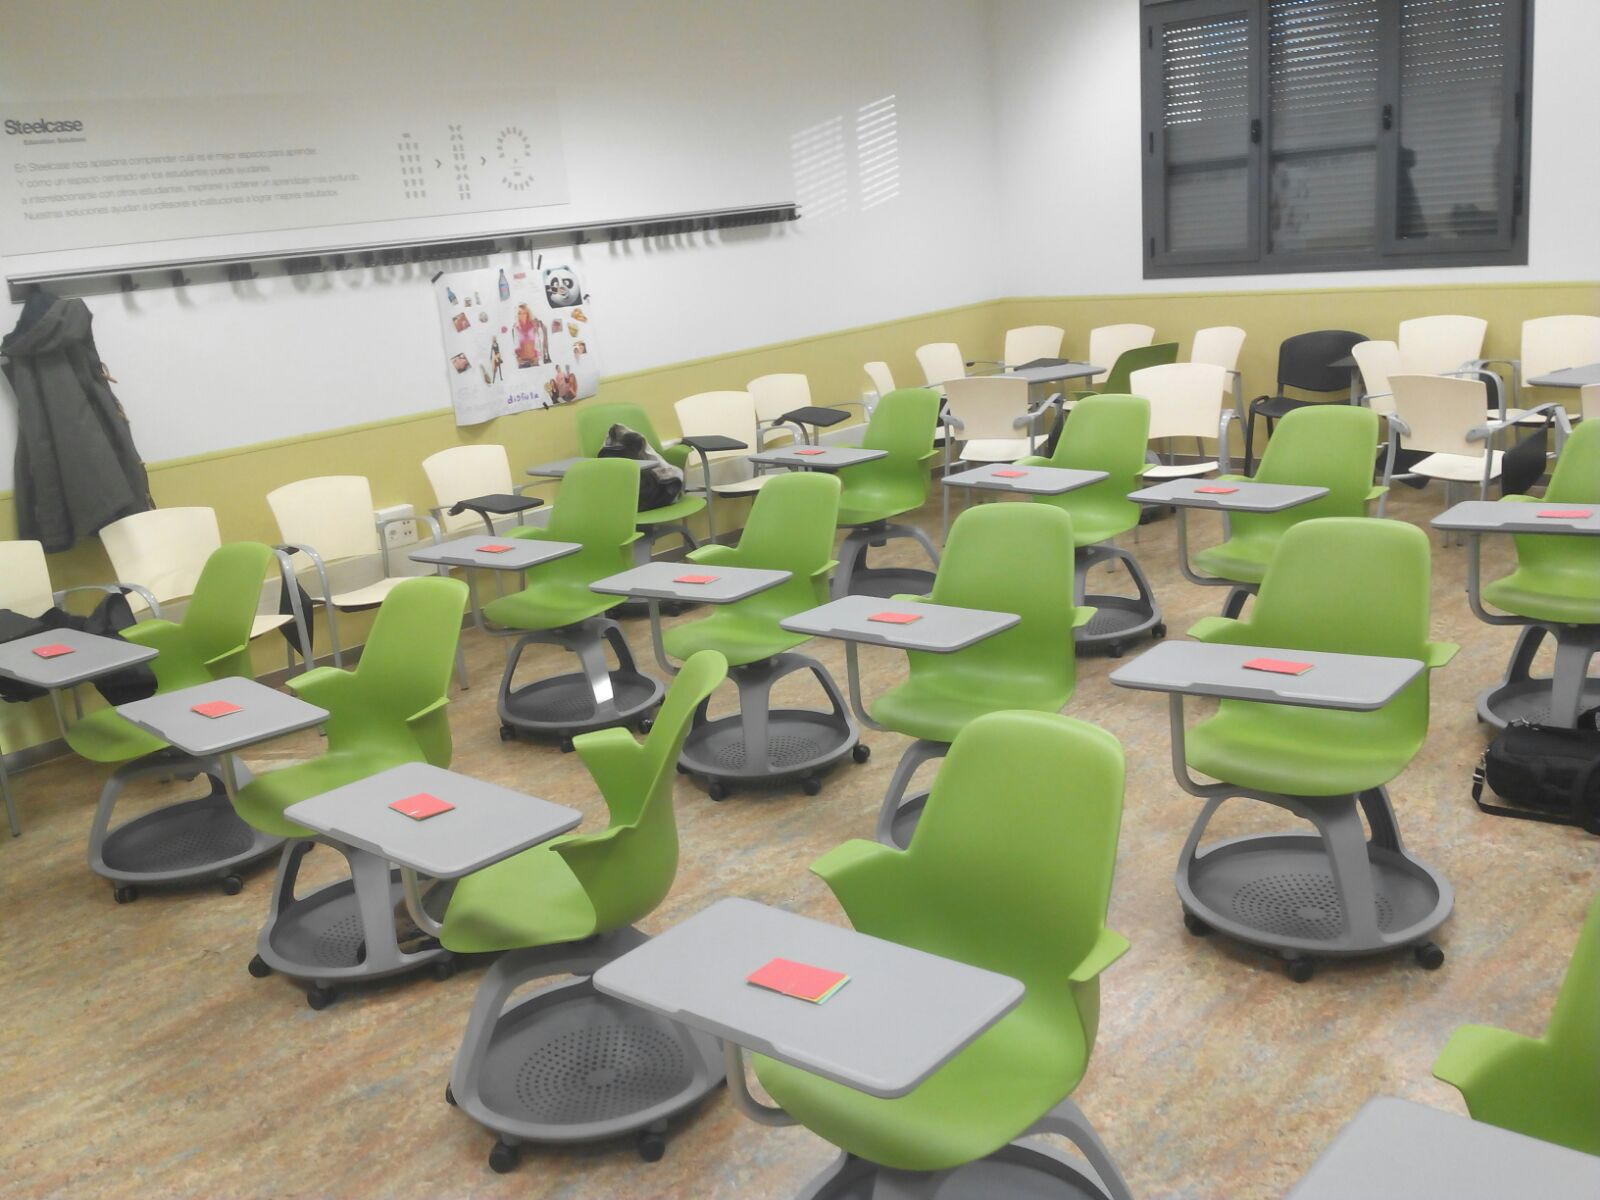
\includegraphics[scale=0.25]{img/clase.jpeg}
\caption{Clase con los sobres preparados, de tal manera que el grupo control está en la mitad izquierda y el experimental a la derecha.}
\label{imgclase}
\end{figure}


Una vez desarrollado el experimento, tendremos un rato de comentar la experiencia. 
%
Pediremos perdón por la pequeña "manipulación", ya que no todos tenían las mismas palabras y preguntaremos al grupo experimental cómo se han sentido.

\paragraph{Resultado en clase:} Muchos de los miembros del grupo \textit{experimental} manifestaban que se habían sentido impotentes e inútiles, llevándoles a no ser capaces de concentrarse para el último sobre.

Como decíamos anteriormente, una vez terminado el experimento en clase, procedemos a explicar el concepto, cómo se detecta y damos algunas herramientas para ponerle solución. 
%
Para más información sobre estos puntos, consultar la presentación de la exposición.

%{\LARGE \textcolor{red}{¿Incluir más descripción?}}

\subsection{Motivación}

Es en este punto de la clase donde arremetemos contra las ideas preconcebidas que puedan tener los alumnos sobre las Matemáticas y su relación con ellas. 
%
Lo ideal sería que empezaran el curso convencidos de que van a sacar las Matemáticas, igual que todas las demás, incluso, con buena nota.
%
Sin embargo, la realidad no suele ser la ideal y es probable que los alumnos hayan tenido problemas con las Matemáticas y crean, desde el primer día, que van a suspenderla.
%
Entablaremos un diálogo sobre su percepción de las Matemáticas, si creen que van a suspender y si se sienten identificados con la indefensión aprendida. Tal vez alguno detecta que le ha ocurrido.

Una vez finalizado, procederemos a dar una visión de las Matemáticas algo distinta a lo habitual: \textbf{las Matemáticas tratan de perspectivas}. 
%
Daremos varios ejemplos de cómo una misma situación tiene muchas perspectivas y como las Matemáticas llevan esto al extremo. 
%
Por poner un ejemplo, el número $\rfrac{4}{3}$ se puede representar de muchísimas maneras distintas, cambiando el sistema de representación, utilizando propiedades físicas, sonidos, etc. 
%
Algunos de estos ejemplos se encuentran en el vídeo de la presentación, obtenido de la charla de Roger Antonsen, \textit{Math is the hidden secret to understanding the world } (TED,2016).

Pondremos también ejemplos reales de perspectivas y de cómo jugar con estadísticas. 
%
En concreto, estos ejemplos versan sobre los datos de paro y resultados electorales publicados en medios de comunicación.
%
En las gráficas propuestas se observan incoherencias.


¿Qué relación tiene esto de perspectivas con estos alumnos? Son ellos quienes, en unos años, serán periodistas, economistas, incluso estadísticos y será su trabajo ser fiel a las representaciones de un mismo hecho e intentar aportar la mejor perspectiva posible. ¡Qué responsabilidad!

Por último, brevemente, indicaremos algunos de los problemas que se van a tratar en la asignatura a lo largo del año.
%
Estos son: optimización de los recursos para maximizar el beneficio (Optimización lineal), el concepto de normalidad y la predicción de variables que se distribuyen normalmente.

\subsection{Método Montecarlo para calcular π}
\label{pimanual}

Éste método se basa en la generación de números aleatorios para aproximar expresiones matemáticas complejas. 
%
El método se llamó así en referencia a la "capital del azar", el casino de Montecarlo.


Dividiremos a la clase por los grupos habituales de trabajo y les daremos a cada uno una cartulina cuadrada con pequeñas paredes y una circunferencia tangente a los lados del cuadrado pintada en el interior. Además, les entregaremos un puñado de arroz de unos 120 granos.
%
En la figura \ref{imgcartulinas} se puede ver el material preparado para ser entregado.

\begin{figure}[hbtp]
\centering
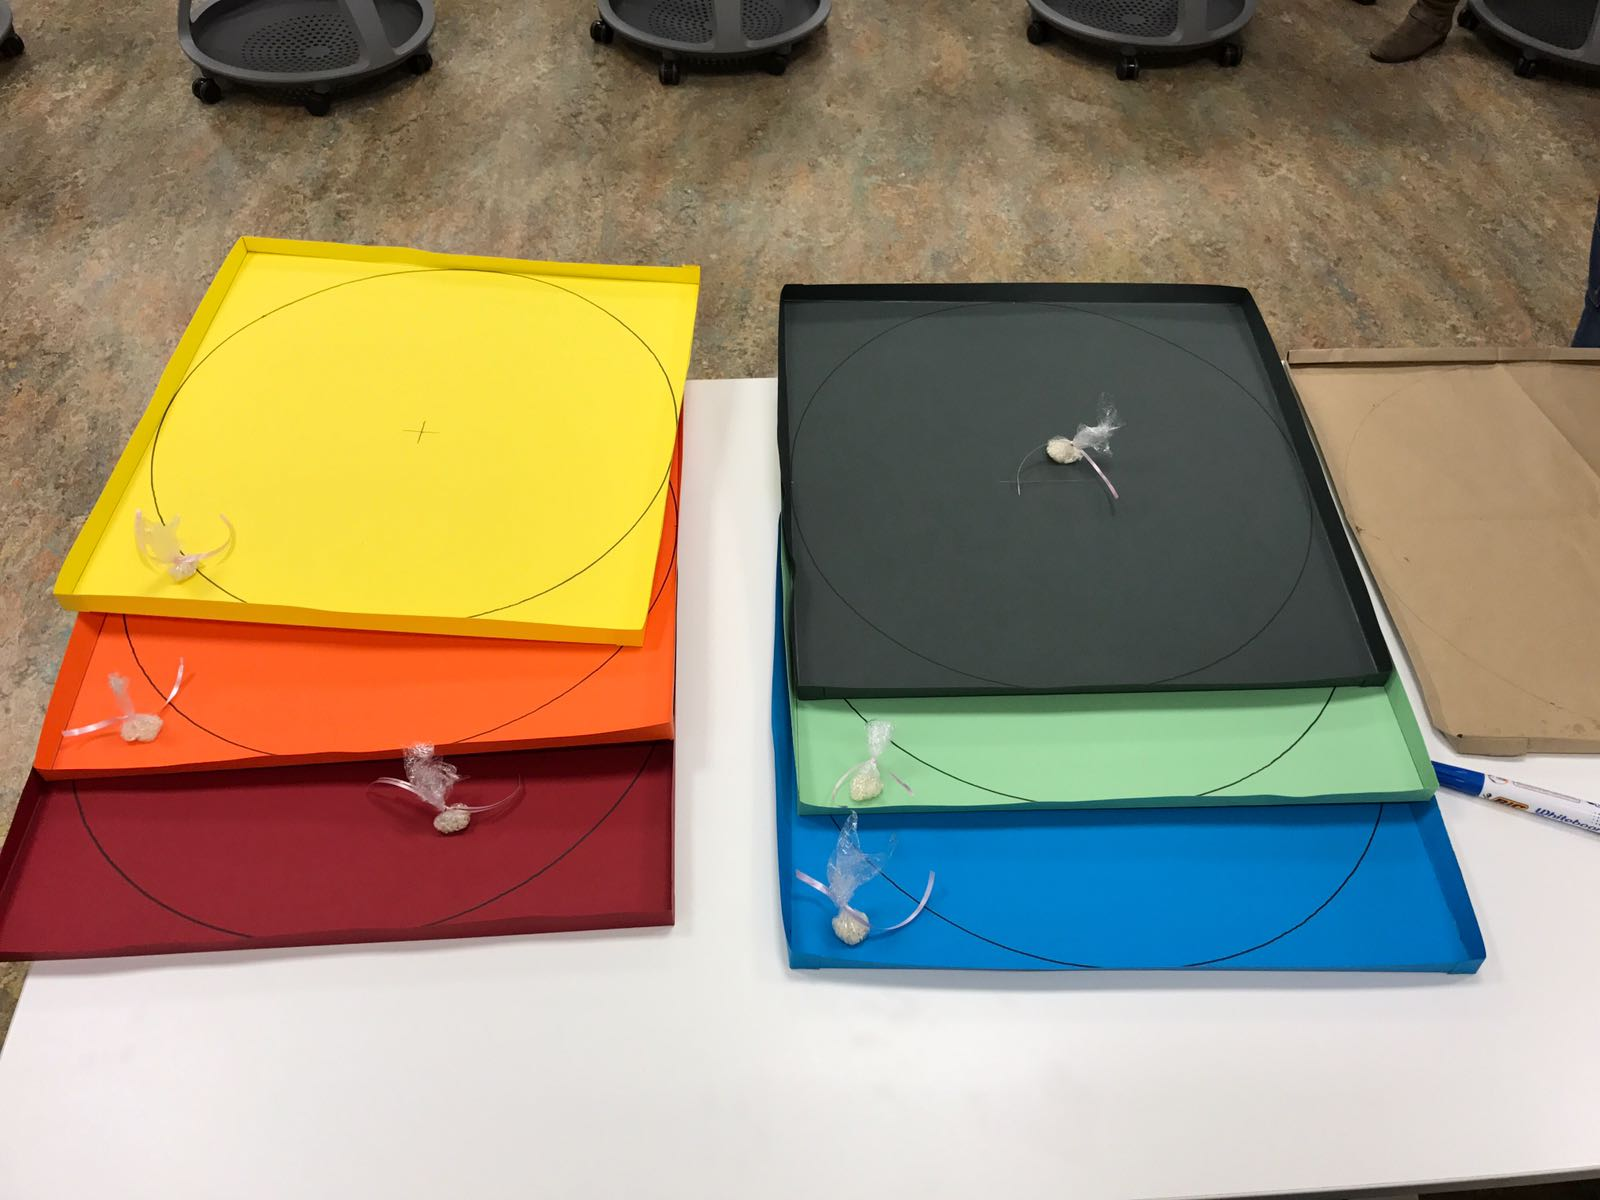
\includegraphics[scale=0.25]{img/cartulinas.jpeg}
\caption{Material preparado para ser entregado a cada grupo. 1 cartulina y una bolsita de arroz con 120 granos por equipo.}
\label{imgcartulinas}
\end{figure}

Un miembro del grupo lanzará el arroz sobre la cartulina y contarán el número de granos que han caído en el círculo y el número de granos que han caído en el cuadrado.
%
Sea $n_{cir}$ el número de granos en el círculo y $n_t$ el número de granos que han caído dentro del cuadrado (algunos de los cuales habrán caído dentro del círculo también).
%
Tendrán que realizar el cálculo $\rfrac{n_{cir}}{n_t}·4$.
%
El número que debería salir sería π. La demostración se encuentra en la figura \ref{imgpidemo}.

\begin{figure}[hbtp]
\centering
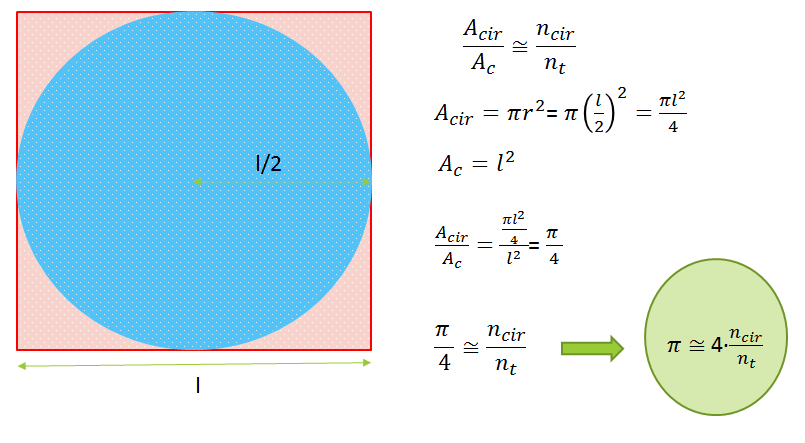
\includegraphics[scale=0.5]{img/pidemo.png}
\caption{Demostración de la relación entre la proporción de granos de arroz y el número π.}
\label{imgpidemo}
\end{figure}

\subsubsection{Limitaciones del experimento:}

Es probable que cada resultado obtenido no se acerque al número π. Esto se debe a algunos factores:

\label{ProblemasExperimento}
\begin{itemize}
	\item Los granos de arroz no se distribuyen uniformemente sobre la cartulina, es decir, no hemos generado puntos suficientemente aleatorios para realizar el experimento.
	\item El número de granos de arroz puede resultar insuficiente. Si cubriéramos absolutamente toda la superficie de la cartulina de granos de arroz, el cálculo sería mucho más exacto.
\end{itemize}

Debido a estos 2 factores, el método de Montecarlo consiste en realizar el experimento muchas veces y tomar la media y la distribución de los resultados obtenidos.

\paragraph{Resultado en clase:} Les propusimos hacer 4 lanzamientos por equipo y calcular la media de los resultados obtenidos. 
%
La mejor media fue $3.22$ y la peor fue $3.81$. 
%
Ninguno de los 2 resultados se acerca mucho, debido a los factores mencionados anteriormente.


\subsubsection{Simulación}

Por lo expuesto en \ref{ProblemasExperimento}, recurrimos a la tecnología, para realizar simulaciones.

Hemos programado un software en $R$ para realizar la simulación de tirar $n$ granos de arroz $m$ veces y estudiar la distribución.
%
Incluimos una imagen del histograma de uno de los resultados obtenidos utilizando $n=100$ y $m=10^5$ (Imagen \ref{imgpidist}). 

En la imagen se puede ver que alguno de los resultados obtenidos era cercano a $2.5$.
%
Es decir, el valor de π aproximado con 100 granos de arroz ha llegado a ser 2,5, una aproximación realmente mala.
%
Por este motivo es tan importante realizar la simulación muchas veces y estudiar la media y la distribución.
%
Se puede observar también que la distribución de los puntos es una distribución normal o gaussiana.

\begin{figure}[hbtp]
\centering
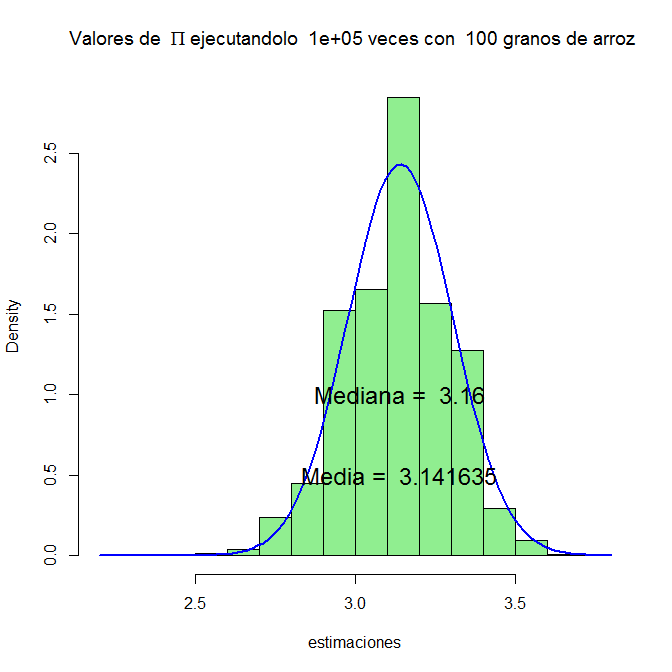
\includegraphics[scale=0.5]{img/piimagen.png}
\caption{Distribución de los valores obtenidos con $n=100$ y $m=10^5$.}
\label{imgpidist}
\end{figure}

\newpage
\section{Fuentes consultadas}

\begin{enumerate}
\item José María Sorando Muzás, \textit{Matemáticas en el debate Zapatero - Rajoy} (2008) [\url{http://catedu.es/matematicas_mundo/SOCIEDAD/sociedad_debate.htm}]
\item Josu Mezo, \textit{El peor gráfico para el peor resultado} (2015) [http://www.malaprensa.com/2015/06/el-peor-grafico-para-el-peor-resultado.html]
\item Will Smith, \textit{Pursuit of happiness} (2012).
\item Roger Antonsen, \textit{Math is the hidden secret to understanding the world } (TED,2016) [\url{https://www.youtube.com/watch?v=70WYy6qZHN4}]
\item Raúl Vaquerizo, \textit{Simulación. Estimación de pi con el método Montecarlo } [\url{http://analisisydecision.es/simulacion-estimacion-de-pi-con-el-metodo-montecarlo}]
\end{enumerate}

\section{Reflexión y autoevaluación}


\subsection{Autoevaluación}

Creemos que hay 2 aspectos fundamentales sobre los que autoevaluarnos. 
%
El primero, sobre el planteamiento del trabajo: el tema escogido, los objetivos y la idea para llevarlos a cabo.
%
El segundo, el desarrollo de la idea en la exposición en clase.

\subsubsection{Planteamiento}

Creemos que el tema elegido es un tema muy importante.
%
Hay muchos alumnos que se sienten indefensos ante las matemáticas, impotentes y así es muy difícil que puedan aprender Matemáticas y utilizarlas. Creemos que el primer paso es atajar esa negatividad.

Los objetivos específicos planteados creemos que están bien alineados con el objetivo general. 
%
Además, aportan una buena estructura para desarrollar la exposición.

Creemos que la manera en la que llevamos a cabo los objetivos fue adecuada, tocando muchos puntos distintos para captar la atención y animar a mantener la concentración: 
\begin{itemize}
	\item El experimento se desarrolla a base de un ejercicio sobre algo que, a priori, no tiene nada de matemáticas (podríamos decir que es un ejercicio rompedor)
	\item Utilización de recursos audiovisuales (presentacíón de PowerPoint, fragmentos audiovisuales)
	\item Utilización de las matemáticas en la vida real (Debate Rajoy-Zapatero).
	\item Material manipulativo.
	\item Nuevas tecnologías (simulación por ordenador).
\end{itemize}

Vemos muy positivo el amplio rango de recursos que se utilizan en este trabajo y además creemos que todos ellos tienen sentido, que no los utilizamos \textit{por utilizar}, sino que de verdad estaban bien enfocados y alineados con los objetivos.

Por comentar un aspecto del planteamiento que, tal vez, es mejorable sería la elección del experimento de montecarlo.
%
Tal vez si realizáramos el experimento de Montecarlo con otro fin distinto a aproximar el número π, los alumnos podrían disfrutarlo más.

Por mencionar un aspecto negativo, del que nos dimos cuenta gracias a las evaluaciones, es que la simuación del experimento de Montecarlo utilizando \textit{R} hace que pueda haber compañeros del máster que no quieran utilizar esta idea en su totalidad, ya que esa parte les resulta más complicada.
%
De todas formas, la simulación se puede realizar con otros programas que pueden estar más al alcance de cualquier docente.

\subsubsection{Desarrollo}

El desarrollo de la exposición se llevó a cabo satisfactoriamente.
%
Creemos que se cumplieron los objetivos:
\begin{itemize}
	\item \textbf{Indefensión aprendida:} hubo alumnos que confirmaron que se habían sentido impotentes y que, debido a los 2 fallos previos, ya no eran capaces de hacer la tercera.
	\item \textbf{Introducción del curso y Motivación:} las evaluaciones recibidas de nuestros compañeros eran positivas en cuanto a que supimos captar la atención de los supuestos alumnos y despertado interés sobre la asignatura.
	\item \textbf{Experimento de Montecarlo:} salió de los propios alumnos que el número que intentábamos aproximar era el número pi.
	%
	En las evaluaciones valoraban positivamente el experimento de Montecarlo, como dinámico y entretenido.
\end{itemize}

Por otro lado, en aspectos a mejorar: nos excedimos de los 40 minutos en el tiempo de la exposición. 
%
Aunque teníamos el planning y habíamos ensayado, en el momento del directo nos alargamos con los tiempos, provocando que el grupo siguiente al nuestro tuviera que hacer su exposición con cierta prisa.

\subsection{Reflexión}

Para la elección del tema se hizo una tormenta de ideas y luego decimos en conjunto cuál se elegía por lo que todos estuvimos de acuerdo y contentos con el tema expuesto.
%
Con la primera parte del trabajo queríamos motivar a los alumnos a que todos pueden hacer aquello que se proponen y quitarles esa indefensión aprendida a las matemáticas.
%
Con la segunda parte queríamos realizar algún tipo de juego de forma que aplicáramos unos de los recursos vistos en clase como son las matemáticas manipulativas.
%
Si bien es cierto, tuvimos dificultades con la elección del material para aplicar el método de Montecarlo ya que en principio la idea era hacer una diana en la pizarra y tirar tizas, pero comprobamos que eso no obtenía los resultados esperados.
%
Finalmente se optó por las cartulinas, aunque por la disposición de la clase sin mesas apropiadas donde apoyarlas también resultó algo peor de los que esperábamos.
%
No obstante, creemos que la idea quedo clara: \textit{motivación y utilidad de las matemáticas en el campo de las ciencias sociales}.

En general estamos bastante satisfechos con el resultado del trabajo, aunque los experimentos podrían haber salido mejor. 
%
El experimento de la indefensión aprendida no funcionó a la perfección, ya que hubo participantes que después de no haber conseguido las 2 primeras, sí consiguieron la última en un tiempo similar a los que habían conseguido las 2 primeras.
%
Sin embargo, el experimento evidenció el efecto que queríamos tratar, con lo que se cumplió el objetivo.
%
Además, nos hubiera gustado que los resultados del juego hubieran sido más próximos al número pi.






\chapter{Valoración de otros trabajos}


\section{Grupo 1 - Cluedo matemático (21/11/2016)}

El primer grupo está formado por:
\begin{itemize}
\item Ana Reyes Camacho 

\item Antonio Jesús Guerrero Lobato 

\item Clara Rocío Lambas Magron 

\item Manuel Pulido Lopez 
\end{itemize}
\begin{figure}[h]
\centering
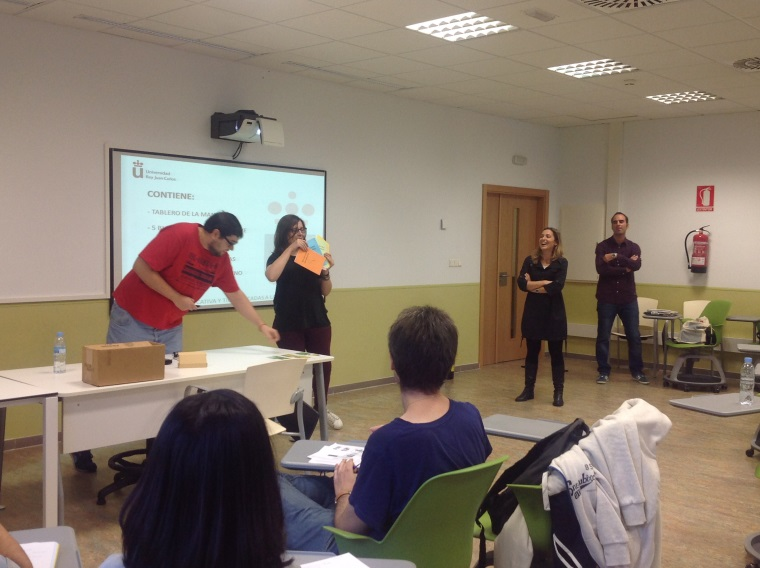
\includegraphics{img/cluedo1.jpg}
\end{figure}
La exposición estaba contextualizada en una clase para alumnos de 1º de la ESO de un IES el último día de clase antes de las vacaciones de Navidad. Durante la clase se tratará la unidad didáctica de la divisibilidad de los números primos y compuestos según aparece en el BOCM. Esta unidad didáctica suele generar mucha confusión entre los alumnos de la ESO y el grupo expositor considera que puede ser de gran interés para el alumnado.

Durante la clase se realizará un juego en el que se formarán varios equipos. Se trata de responder a una serie de preguntas en las que se premiará la rapidez en las respuestas siempre y cuando sean correctas. Por un lado el juego permitirá captar la atención de los alumnos. Por otro, el trabajo en equipo fomenta los valores de colaboración con los compañeros y el hecho de que sean preguntas cronometradas permitirá a las alumnas adaptarse a condiciones de trabajo de ciertas “presión”.

El juego se titula “Cluedo matemático”. El enunciado del juego dice así:

¡Esta noche el Señor Cero ha sido hallado asesinado en su mansión! Los detectives privados Simple y Compuesto han encontrado 99 sospechosos, pero no han podido resolver el caso. ¡Así que ahora la resolución del crimen depende de vosotros! Para ganar el juego debéis averiguar una sola cosa sobre el crimen”

Para la preparación del juego se:
\begin{itemize}
\item[1.] Coloca el tablero, hay un Hall donde empieza la acción y donde se coloca el peón, y 5 habitaciones dónde buscar pistas.

\item[2.] Prepara las tarjetas de preguntas, un tema para cada habitación.

 \item[3.] Prepara las tarjetas de pistas para descubrir al asesino, un pack de pistas por cada equipo.

\item[4.] Organiza a los alumnos en grupo, nombrando un portavoz
\end{itemize}

 \begin{figure}[h]
 \centering
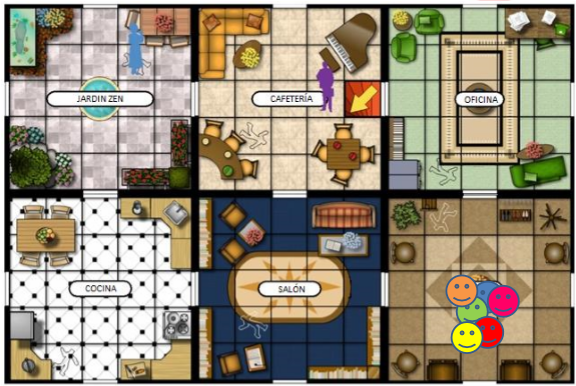
\includegraphics[scale=0.6]{img/cluedo2.jpg}
\end{figure}

Las reglas del juego son:
\begin{itemize}
\item[1.] CÓMO GANAR: ¡Resuelve el crimen!  

\item[2.] CÓMO JUGAR: En cada turno se mueve el peón a una habitación contigua, se le hace a todos los grupos la misma pregunta, se dejan 120'' para calcular la respuesta y si contestan correctamente se les da una pista sobre el asesino.

\begin{figure}[h]
\centering
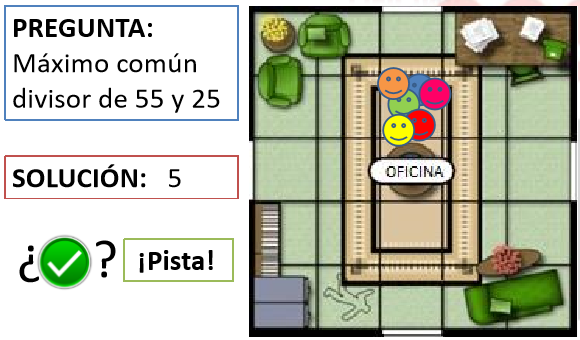
\includegraphics[scale=0.6]{img/cluedo3.jpg}
\end{figure}

\end{itemize}

 
La función principal del juego consistía en hacer preguntas por grupos y había que averiguar el número comprendido entre el 1 y el 99 a partir de una serie de pistas que se iban consiguiendo.

La exposición del grupo estuvo muy bien estructurada y demostraron que hicieron un gran trabajo de equipo.

Durante la misma explicaron que desestimaron la opción de tirar un dado, pero nosotros sí lo habríamos incluido incluyendo la posibilidad de que hubiese un rebote al tener un cronometro. Pero la opción del rebote también la descartaron.

La dificultad de las preguntas era variable por lo que es un juego muy versátil y de alto valor añadido para el aprendizaje.

Nos sorprendieron con algo novedoso al proponer analizar y evaluar el juego al final de la clase, lo que les permitirá que hubiese una mejora continua con los años. Para esta evaluación pidieron a los alumnos que contestaran a una serie de preguntas sobre lo que les ha parecido. Aunque sabemos que es difícil discernir cuando la exposición la realizas en el contexto de alumnos de secundario o en el contexto nuestro de alumnos de master, bajo nuestro punto de vista quizá sea demasiado pronto pedir la opinión a un niño de 1º de la ESO su opinión.

La exposición se ha ajustado perfectamente a los tiempos programados.


\section{Grupo 2 - Construyendo las matemáticas (21/11/2016)}


El segundo grupo está formado por:
\begin{itemize}
\item Helena Matesanz Marín 

\item Cristina Martínez Gonzalez 

\item Eliseo Virseda Alvaro 

\item Noemi Castillo Cumplido 

\item David Soria Castro 
\end{itemize}

\begin{figure}[hbtp]
\centering
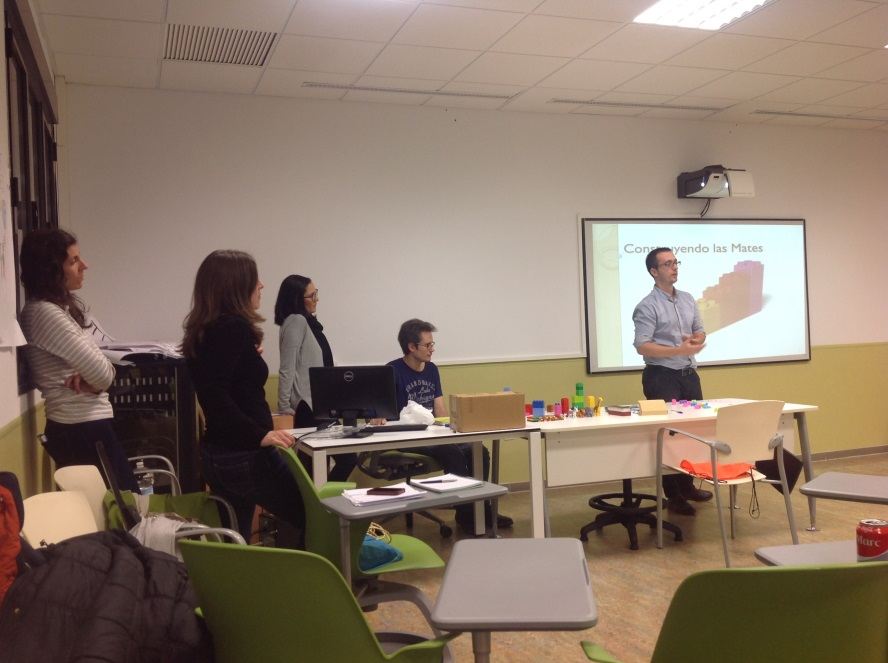
\includegraphics[scale=1]{img/lego1.jpg}
\caption{Integrantes del grupo 2.}
\end{figure}

 
La exposición consistió en explicar con un material manipulativo conocido por los alumnos, que son las piezas de LEGO, los siguientes conceptos matemáticos que en el papel pueden parecer abstractos. Los conceptos matemáticos mostrados fueron:
\begin{itemize}
\item Fracciones 

\item Estadística 

\item Máximo común divisor y mínimo común múltiplo 

\item Ecuaciones lineales simples. Despejar la x. 

\item Teorema de Pitágoras 
\end{itemize}

\begin{figure}[hbtp]
\centering
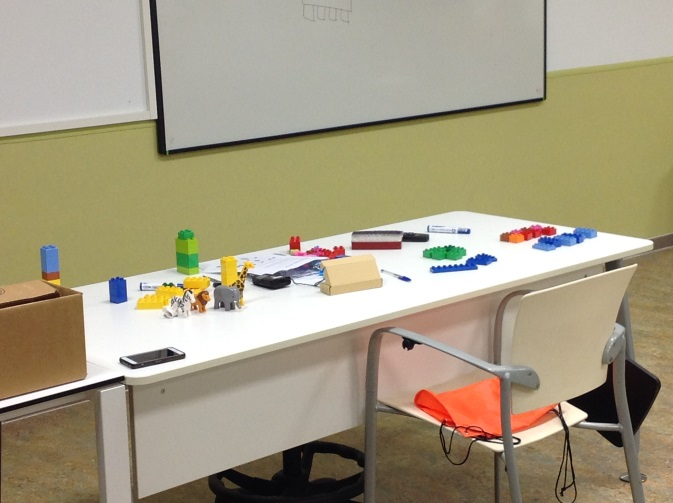
\includegraphics[scale=1]{img/lego2.jpg}
\caption{Materiales manipulativos.}
\end{figure}
 
En nuestra opinión el uso de LEGO para varios conceptos matemáticos hizo que algunos de estos temas estuvieran un poco forzados. Es decir, para el concepto de fracciones las piezas de LEGO fueron de gran utilidad al permitir de una manera visual entender el concepto de lo que es una fracción como una parte de un todo. Sin embargo consideramos que explicar el concepto de M.c.d y m.c.m con piezas de LEGO quedó un poco forzado.

Por hacer una crítica constructiva, entendemos que era un grupo de 5 alumnos, es decir, de más alumnos que el resto de grupos de clase, pero quizá hubiésemos enfocado el trabajo en uno o dos conceptos matemáticos y habríamos trabajado un par de alumnos por cada concepto para evitar explicaciones de conceptos forzadas.

La exposición estuvo muy bien estructurada con una demostración conceptual por cada alumno pero se fueron de tiempo. Es cierto que se han explicado muchos conceptos pero los alumnos no hemos colaborado con lo que se puede perder eficacia al no hacer partícipes a los alumnos. Pero también entendemos que todos tenían que hablar y que eran temas muy interesantes.

Por último, la exposición también nos sirvió para aprender que a día de hoy hay un software en una web de internet (\url{http://www.publishyourdesign.com/}) que te permite realizar diseños de LEGO en 3D con el ordenador para luego poder incluso imprimirlos con impresoras 3D.


\section{Grupo 4 - La Oca Matemática (28/11/2016)}

Integrantes del grupo:

\begin{itemize}

\item Óscar Abelda
\item Miriam Expósito
\item Beatriz Mate
\item Pablo Saiz
\end{itemize}

\begin{minipage}[hbtp]{1.0\linewidth}
\centering
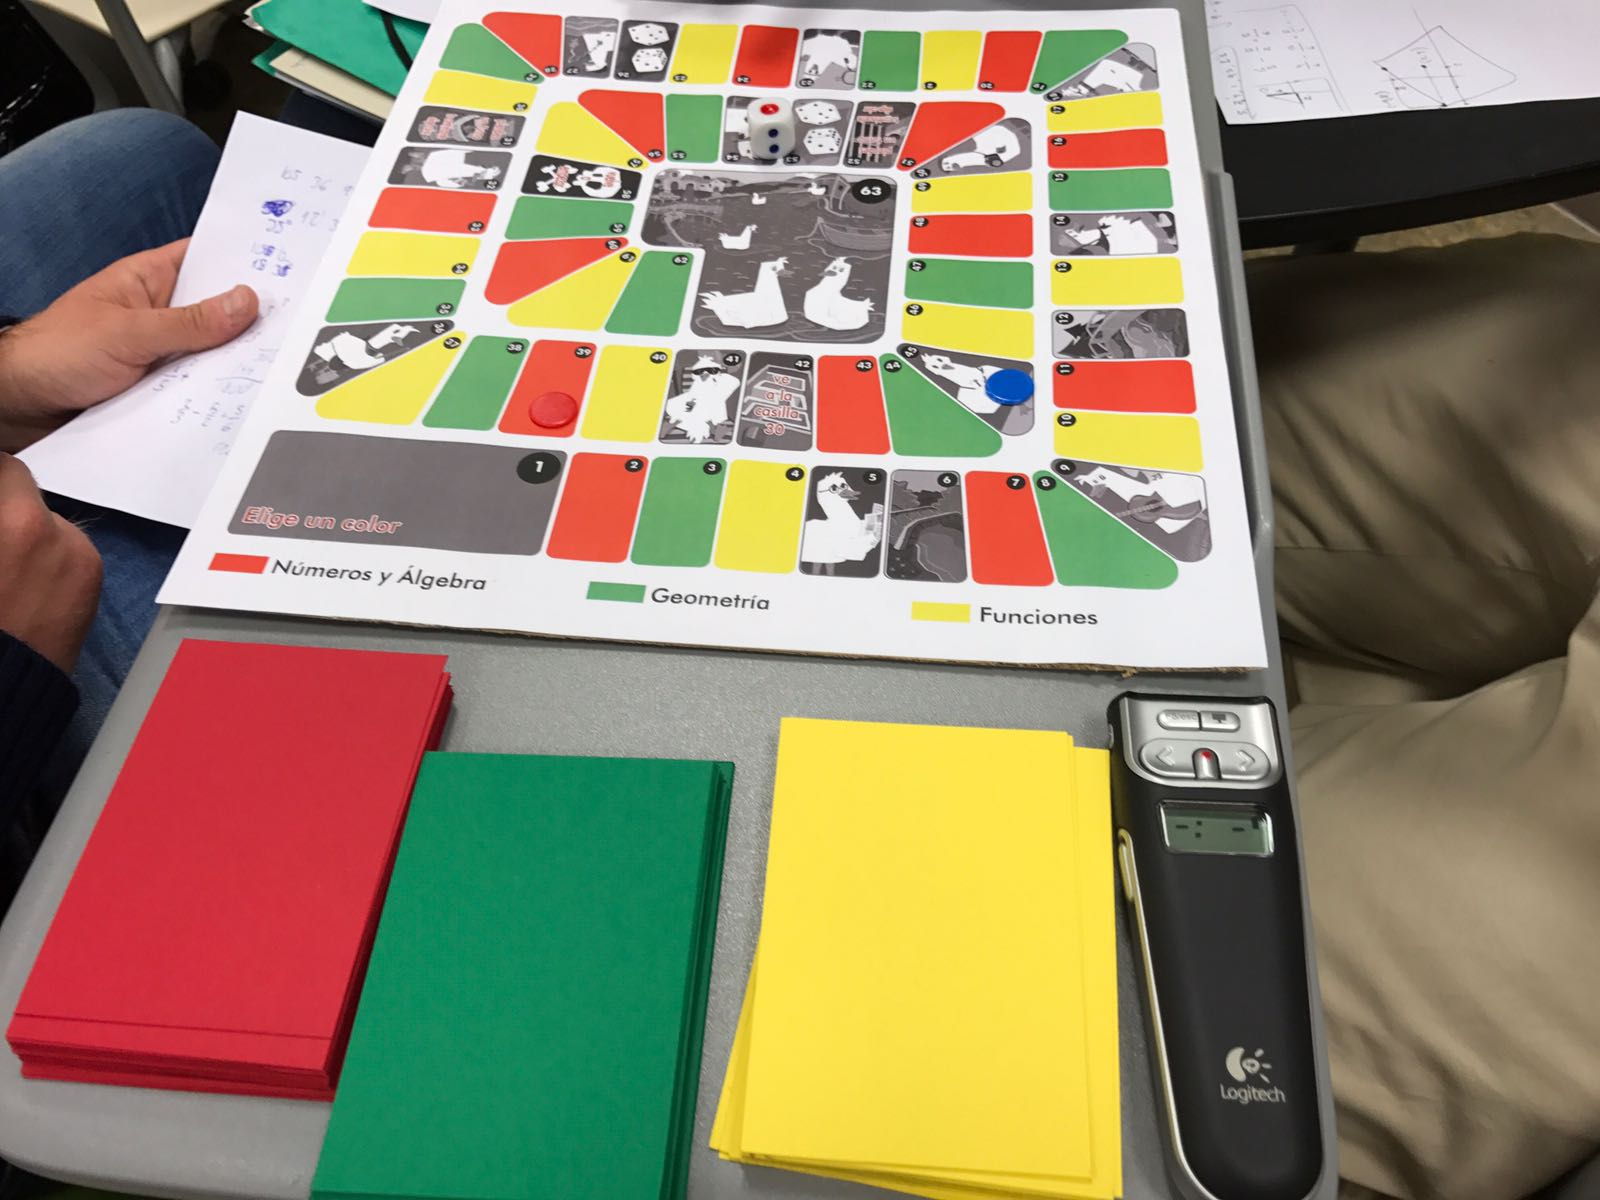
\includegraphics[scale=0.2]{img/grupo4_1.jpg}
\captionof{figure}{Material para cada grupo}.
\end{minipage}

Se presentó un juego clásico rediseñado para su aplicación en el campo de las matemáticas de 2º de la ESO. Desde un principio han sido capaces de meternos en el contexto de la situación en la cual sería aplicable la actividad. Está orientada a ese último día de clase donde podemos repasar contenidos de forma lúdica, sin que resulte aburrido para el alumnado. 

Nos sorprendió gratamente el gran trabajo realizado a la hora de elaborar el material manipulativo. La actividad contenía las instrucciones del juego, dado, tablero, tarjetas de contenidos, fichas, etc. Estábamos ante un juego de sobremesa con todo tipo de detalles.

Al poco tiempo de comenzar el juego, nos dimos cuenta de que pese a nuestra edad, poco a poco se iba incrementando la competitividad entre nosotros. No parábamos de comprobar si la pareja opuesta estaba resolviendo bien las preguntas, tiempo empleado, cuáles eran sus materias fuertes, etc. En todo momento contamos con un supervisor del grupo autor del juego, que nos guió durante la actividad.








%% Apendices (ejercicios, examenes)
%\appendix

%\chapter{---}% -*- root: ../Innovacion.tex -*-

\section{Conglomerado de recursos}

\begin{itemize}
	\item
	Estudios internacionales de Evaluación
	http://www.mecd.gob.es/inee/publicaciones/estudios-internacionales.html 
	\item 
	Instituto NAcional de Tecnologias Eduativas y Formación del profesorado 
	http://educalab.es/intef
	\item 
	Seamos gansos
	https://www.youtube.com/watch?v=K5G8gRvx7nQ
	\item 
	9 gestos cotidianos que los matemáticos hacemos de otra manera:
	http://verne.elpais.com/verne/2015/11/13/articulo/1447413460_147289.html?id_externo_rsoc=FB_CM
	\item 
	La escuela en 2030
	http://www.elmundo.es/espana/2014/10/21/54455b9f22601d22738b458e.html
	\item 
	El cerebro necesita emocionase para aprender
	http://economia.elpais.com/economia/2016/07/17/actualidad/1468776267_359871.html
	\item 
	La neuroeducación demuestra que emocion y conocimiento van juntos
	http://blogs.elpais.com/ayuda-al-estudiante/2013/12/la-neuroeducacion-demuestra-que-emocion-y-conocimiento-van-juntos.html
	\item 
	mates y neurociencia
	https://escuelaconcerebro.wordpress.com/2012/03/20/matematicas-y-neurociencia/
	\item 
	actividad cerebral del alumno durante la clase magistral
	http://ined21.com/actividad-cerebral-del-alumno-durante-la-tradicional-clase-magistral/
	\item 
	Aprendizaje cooperativo y neuroeducación: guiando la poda sináptica
	https://escuelaconcerebro.wordpress.com/2016/08/18/aprendizaje-cooperativo-y-neuroeducacion-guiando-la-poda-sinaptica/

\end{itemize}


\printindex
\end{document}
